\documentclass[]{ctexbook}
\usepackage{lmodern}
\usepackage{amssymb,amsmath}
\usepackage{ifxetex,ifluatex}
\usepackage{fixltx2e} % provides \textsubscript
\ifnum 0\ifxetex 1\fi\ifluatex 1\fi=0 % if pdftex
  \usepackage[T1]{fontenc}
  \usepackage[utf8]{inputenc}
\else % if luatex or xelatex
  \ifxetex
    \usepackage{xltxtra,xunicode}
  \else
    \usepackage{fontspec}
  \fi
  \defaultfontfeatures{Ligatures=TeX,Scale=MatchLowercase}
\fi
% use upquote if available, for straight quotes in verbatim environments
\IfFileExists{upquote.sty}{\usepackage{upquote}}{}
% use microtype if available
\IfFileExists{microtype.sty}{%
\usepackage{microtype}
\UseMicrotypeSet[protrusion]{basicmath} % disable protrusion for tt fonts
}{}
\usepackage[b5paper,tmargin=2.5cm,bmargin=2.5cm,lmargin=3.5cm,rmargin=2.5cm]{geometry}
\usepackage[unicode=true]{hyperref}
\PassOptionsToPackage{usenames,dvipsnames}{color} % color is loaded by hyperref
\hypersetup{
            pdftitle={Face lab book},
            pdfauthor={Face lab},
            colorlinks=true,
            linkcolor=Maroon,
            citecolor=Blue,
            urlcolor=Blue,
            breaklinks=true}
\urlstyle{same}  % don't use monospace font for urls
\usepackage{natbib}
\bibliographystyle{apalike}
\usepackage{color}
\usepackage{fancyvrb}
\newcommand{\VerbBar}{|}
\newcommand{\VERB}{\Verb[commandchars=\\\{\}]}
\DefineVerbatimEnvironment{Highlighting}{Verbatim}{commandchars=\\\{\}}
% Add ',fontsize=\small' for more characters per line
\usepackage{framed}
\definecolor{shadecolor}{RGB}{248,248,248}
\newenvironment{Shaded}{\begin{snugshade}}{\end{snugshade}}
\newcommand{\AlertTok}[1]{\textcolor[rgb]{0.94,0.16,0.16}{#1}}
\newcommand{\AnnotationTok}[1]{\textcolor[rgb]{0.56,0.35,0.01}{\textbf{\textit{#1}}}}
\newcommand{\AttributeTok}[1]{\textcolor[rgb]{0.13,0.29,0.53}{#1}}
\newcommand{\BaseNTok}[1]{\textcolor[rgb]{0.00,0.00,0.81}{#1}}
\newcommand{\BuiltInTok}[1]{#1}
\newcommand{\CharTok}[1]{\textcolor[rgb]{0.31,0.60,0.02}{#1}}
\newcommand{\CommentTok}[1]{\textcolor[rgb]{0.56,0.35,0.01}{\textit{#1}}}
\newcommand{\CommentVarTok}[1]{\textcolor[rgb]{0.56,0.35,0.01}{\textbf{\textit{#1}}}}
\newcommand{\ConstantTok}[1]{\textcolor[rgb]{0.56,0.35,0.01}{#1}}
\newcommand{\ControlFlowTok}[1]{\textcolor[rgb]{0.13,0.29,0.53}{\textbf{#1}}}
\newcommand{\DataTypeTok}[1]{\textcolor[rgb]{0.13,0.29,0.53}{#1}}
\newcommand{\DecValTok}[1]{\textcolor[rgb]{0.00,0.00,0.81}{#1}}
\newcommand{\DocumentationTok}[1]{\textcolor[rgb]{0.56,0.35,0.01}{\textbf{\textit{#1}}}}
\newcommand{\ErrorTok}[1]{\textcolor[rgb]{0.64,0.00,0.00}{\textbf{#1}}}
\newcommand{\ExtensionTok}[1]{#1}
\newcommand{\FloatTok}[1]{\textcolor[rgb]{0.00,0.00,0.81}{#1}}
\newcommand{\FunctionTok}[1]{\textcolor[rgb]{0.13,0.29,0.53}{\textbf{#1}}}
\newcommand{\ImportTok}[1]{#1}
\newcommand{\InformationTok}[1]{\textcolor[rgb]{0.56,0.35,0.01}{\textbf{\textit{#1}}}}
\newcommand{\KeywordTok}[1]{\textcolor[rgb]{0.13,0.29,0.53}{\textbf{#1}}}
\newcommand{\NormalTok}[1]{#1}
\newcommand{\OperatorTok}[1]{\textcolor[rgb]{0.81,0.36,0.00}{\textbf{#1}}}
\newcommand{\OtherTok}[1]{\textcolor[rgb]{0.56,0.35,0.01}{#1}}
\newcommand{\PreprocessorTok}[1]{\textcolor[rgb]{0.56,0.35,0.01}{\textit{#1}}}
\newcommand{\RegionMarkerTok}[1]{#1}
\newcommand{\SpecialCharTok}[1]{\textcolor[rgb]{0.81,0.36,0.00}{\textbf{#1}}}
\newcommand{\SpecialStringTok}[1]{\textcolor[rgb]{0.31,0.60,0.02}{#1}}
\newcommand{\StringTok}[1]{\textcolor[rgb]{0.31,0.60,0.02}{#1}}
\newcommand{\VariableTok}[1]{\textcolor[rgb]{0.00,0.00,0.00}{#1}}
\newcommand{\VerbatimStringTok}[1]{\textcolor[rgb]{0.31,0.60,0.02}{#1}}
\newcommand{\WarningTok}[1]{\textcolor[rgb]{0.56,0.35,0.01}{\textbf{\textit{#1}}}}
\usepackage{longtable,booktabs}
% Fix footnotes in tables (requires footnote package)
\IfFileExists{footnote.sty}{\usepackage{footnote}\makesavenoteenv{long table}}{}
\usepackage{graphicx,grffile}
\makeatletter
\def\maxwidth{\ifdim\Gin@nat@width>\linewidth\linewidth\else\Gin@nat@width\fi}
\def\maxheight{\ifdim\Gin@nat@height>\textheight\textheight\else\Gin@nat@height\fi}
\makeatother
% Scale images if necessary, so that they will not overflow the page
% margins by default, and it is still possible to overwrite the defaults
% using explicit options in \includegraphics[width, height, ...]{}
\setkeys{Gin}{width=\maxwidth,height=\maxheight,keepaspectratio}
\IfFileExists{parskip.sty}{%
\usepackage{parskip}
}{% else
\setlength{\parindent}{0pt}
\setlength{\parskip}{6pt plus 2pt minus 1pt}
}
\setlength{\emergencystretch}{3em}  % prevent overfull lines
\providecommand{\tightlist}{%
  \setlength{\itemsep}{0pt}\setlength{\parskip}{0pt}}
\setcounter{secnumdepth}{5}
% Redefines (sub)paragraphs to behave more like sections
\ifx\paragraph\undefined\else
\let\oldparagraph\paragraph
\renewcommand{\paragraph}[1]{\oldparagraph{#1}\mbox{}}
\fi
\ifx\subparagraph\undefined\else
\let\oldsubparagraph\subparagraph
\renewcommand{\subparagraph}[1]{\oldsubparagraph{#1}\mbox{}}
\fi

% set default figure placement to htbp
\makeatletter
\def\fps@figure{htbp}
\makeatother

\usepackage{booktabs}
\usepackage{longtable}

\usepackage{framed,color}
\definecolor{shadecolor}{RGB}{248,248,248}

\renewcommand{\textfraction}{0.05}
\renewcommand{\topfraction}{0.8}
\renewcommand{\bottomfraction}{0.8}
\renewcommand{\floatpagefraction}{0.75}

\let\oldhref\href
\renewcommand{\href}[2]{#2\footnote{\url{#1}}}

\makeatletter
\newenvironment{kframe}{%
\medskip{}
\setlength{\fboxsep}{.8em}
 \def\at@end@of@kframe{}%
 \ifinner\ifhmode%
  \def\at@end@of@kframe{\end{minipage}}%
  \begin{minipage}{\columnwidth}%
 \fi\fi%
 \def\FrameCommand##1{\hskip\@totalleftmargin \hskip-\fboxsep
 \colorbox{shadecolor}{##1}\hskip-\fboxsep
     % There is no \\@totalrightmargin, so:
     \hskip-\linewidth \hskip-\@totalleftmargin \hskip\columnwidth}%
 \MakeFramed {\advance\hsize-\width
   \@totalleftmargin\z@ \linewidth\hsize
   \@setminipage}}%
 {\par\unskip\endMakeFramed%
 \at@end@of@kframe}
\makeatother

\makeatletter
\@ifundefined{Shaded}{
}{\renewenvironment{Shaded}{\begin{kframe}}{\end{kframe}}}
\@ifpackageloaded{fancyvrb}{%
  % https://github.com/CTeX-org/ctex-kit/issues/331
  \RecustomVerbatimEnvironment{Highlighting}{Verbatim}{commandchars=\\\{\},formatcom=\xeCJKVerbAddon}%
}{}
\makeatother

\usepackage{makeidx}
\makeindex

\urlstyle{tt}

\usepackage{amsthm}
\makeatletter
\def\thm@space@setup{%
  \thm@preskip=8pt plus 2pt minus 4pt
  \thm@postskip=\thm@preskip
}
\makeatother

\frontmatter

\title{Face lab book}
\author{Face lab}
\date{2024-11-10}

\usepackage{amsthm}
\newtheorem{theorem}{Theorem}[chapter]
\newtheorem{lemma}{Lemma}[chapter]
\newtheorem{corollary}{Corollary}[chapter]
\newtheorem{proposition}{Proposition}[chapter]
\newtheorem{conjecture}{Conjecture}[chapter]
\theoremstyle{definition}
\newtheorem{definition}{Definition}[chapter]
\theoremstyle{definition}
\newtheorem{example}{Example}[chapter]
\theoremstyle{definition}
\newtheorem{exercise}{Exercise}[chapter]
\theoremstyle{definition}
\newtheorem{hypothesis}{Hypothesis}[chapter]
\theoremstyle{remark}
\newtheorem*{remark}{Remark}
\newtheorem*{solution}{Solution}
\begin{document}
\maketitle


\thispagestyle{empty}

\begin{center}
献给……

\end{center}

\setlength{\abovedisplayskip}{-5pt}
\setlength{\abovedisplayshortskip}{-5pt}

{
\setcounter{tocdepth}{2}
\tableofcontents
}
\listoftables
\listoffigures
\chapter{简介}\label{ux7b80ux4ecb}

这是面孔实验室的实验手册,目前主要尝试介绍一些常用的软件或技术。

实验室目前常用的软件有:

\begin{itemize}
\tightlist
\item
  第 \ref{jamovi} 章: Jamovi\\
\item
  第 \ref{zotero} 章: Zotero
\end{itemize}

\mainmatter

\part{统计软件}\label{part-ux7edfux8ba1ux8f6fux4ef6}

\chapter{Jamovi}\label{jamovi}

汇总:沈佳欣、张宇杰\\
更新于:2024-11-07

\section{方差分析}\label{ux65b9ux5deeux5206ux6790}

导入数据后,依次点击``分析''\,``方差分析''选项,然后在弹出的选项栏中选择适当的方差分析方法。前五个为参数检验方法,后两个为非参数检验方法,它们分别对应统计课本中的克-瓦氏单向方差分析和弗里德曼两因素等级方差分析。

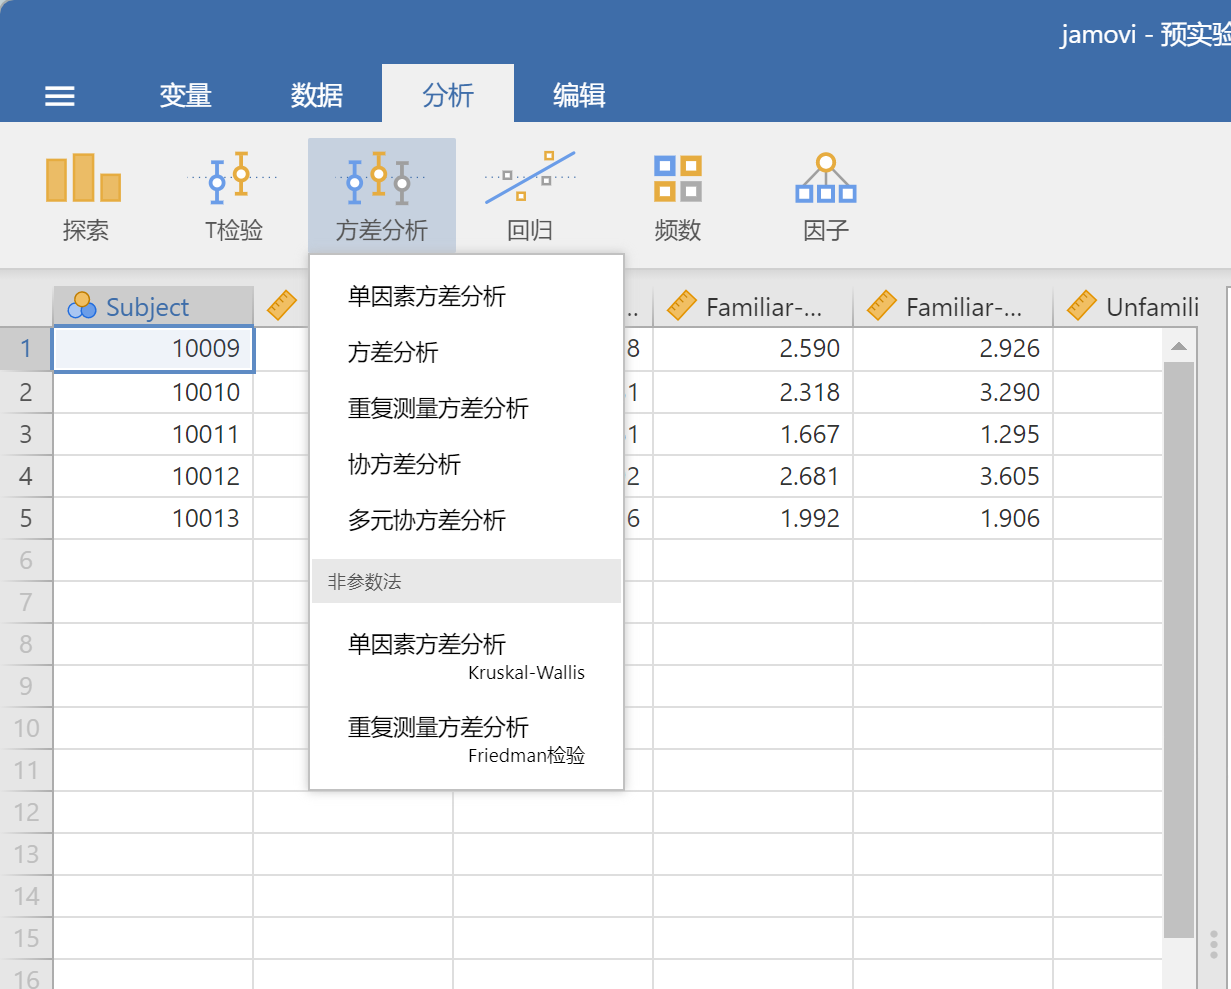
\includegraphics{img/jamovi/anova.png}

此次以重复测量方差分析为例。在下图左侧的界面里,左侧是我们数据的名称,右侧的``重复测量因子''是指在研究中设置的``被试内自变量''。在本例中,我们有三个``被试内自变量'',每个自变量都有两个水平。例如我们将``重复测量因子1''定义为Familiar,它包括``familiar''和``unfamiliar''两个水平。

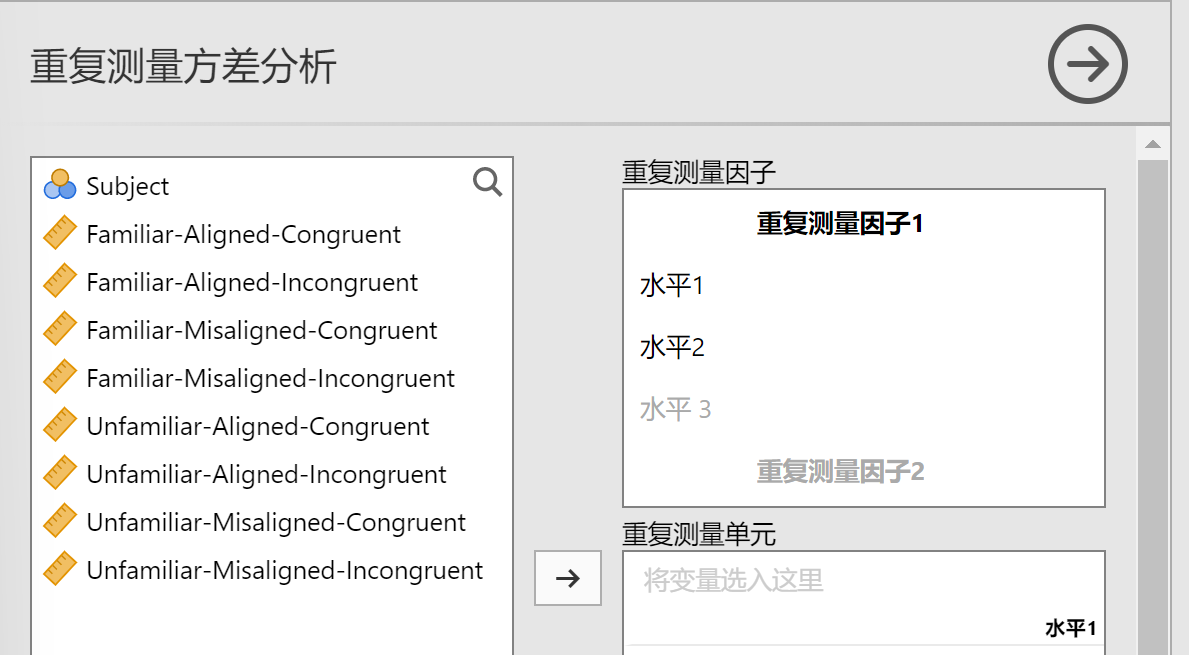
\includegraphics{img/jamovi/rmanova-factor.png}\\
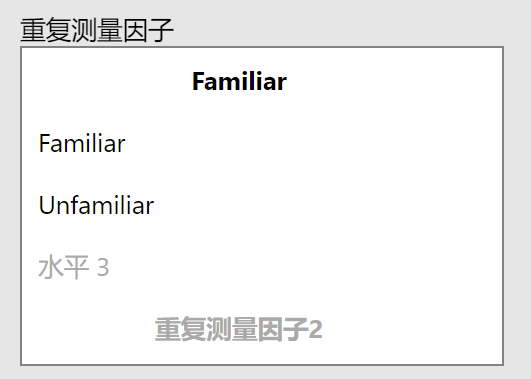
\includegraphics{img/jamovi/rmanova-factorlevels.png}

定义好重复测量因子后,``重复测量单元''中会出现各个自变量水平的组合,而``重复测量单元''也就是指研究中的各种实验条件。在本例中我们的实验是一个2 * 2 * 2的被试内设计,所以共有8种实验条件,我们需要做的是将数据拖入其对应的重复测量单元中。

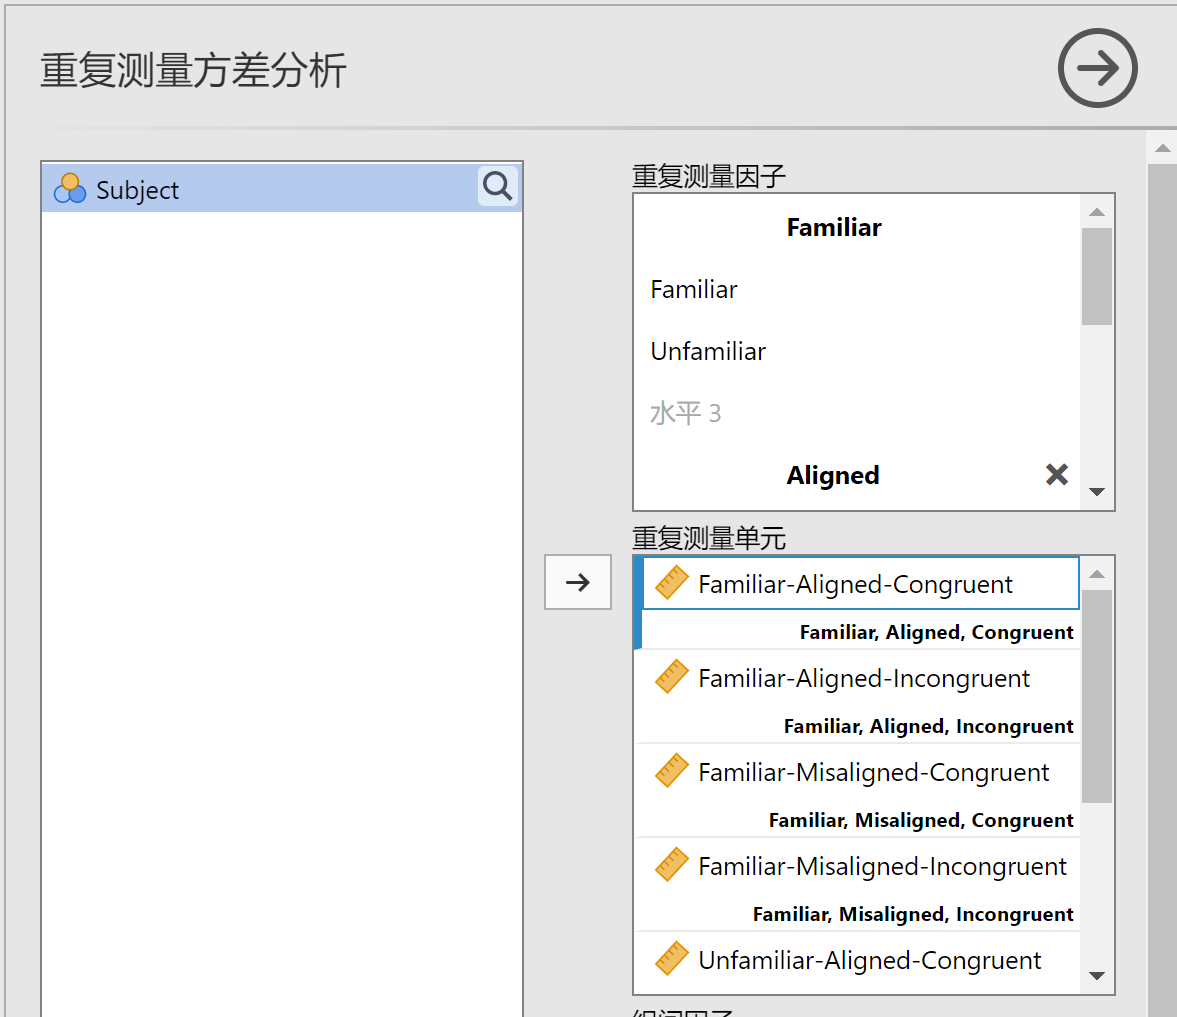
\includegraphics{img/jamovi/rmanova-factorlevels2.png}

接下来我们要选择效应量为``偏η²值'',以及确定因变量标签。本例中因变量标签为``d-prime''.

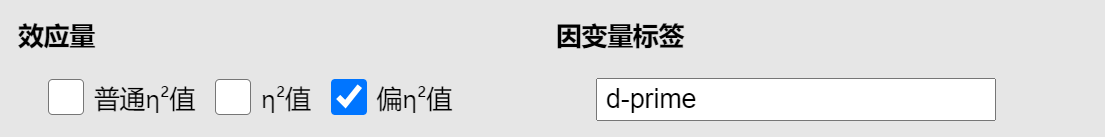
\includegraphics{img/jamovi/rmanova-dv.png}

下面的五个选项里,我们应当关注的主要是``适用条件判断''和``事后检验''。

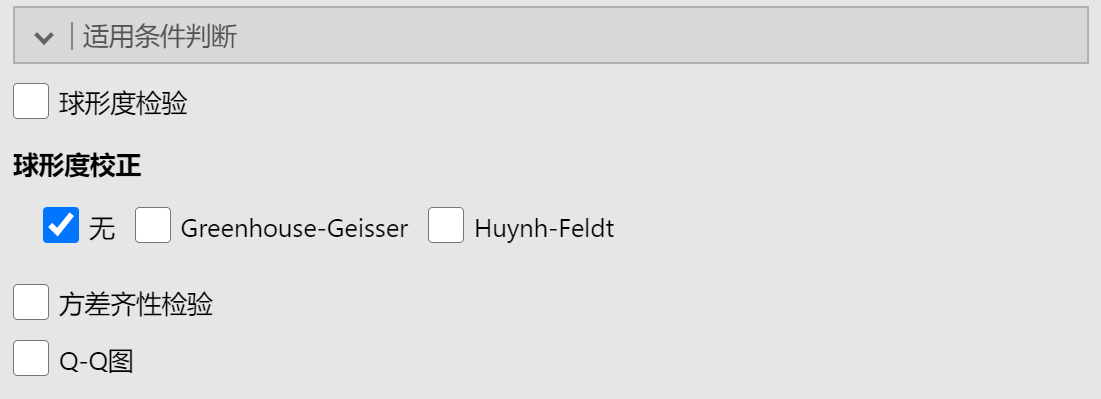
\includegraphics{img/jamovi/rmanova-sphericity.png}

对本专业来说,在这一栏中较为重要的是``方差齐性检验'',如果变量中涉及被试间变量,那么应当进行方差齐性检验。但由于本例中的变量都是被试内变量,所以无需进行方差齐性检验。其他几个选项可以根据研究所需进行选取。

所有设定完成后,jamovi会在右侧呈现数据分析结果。

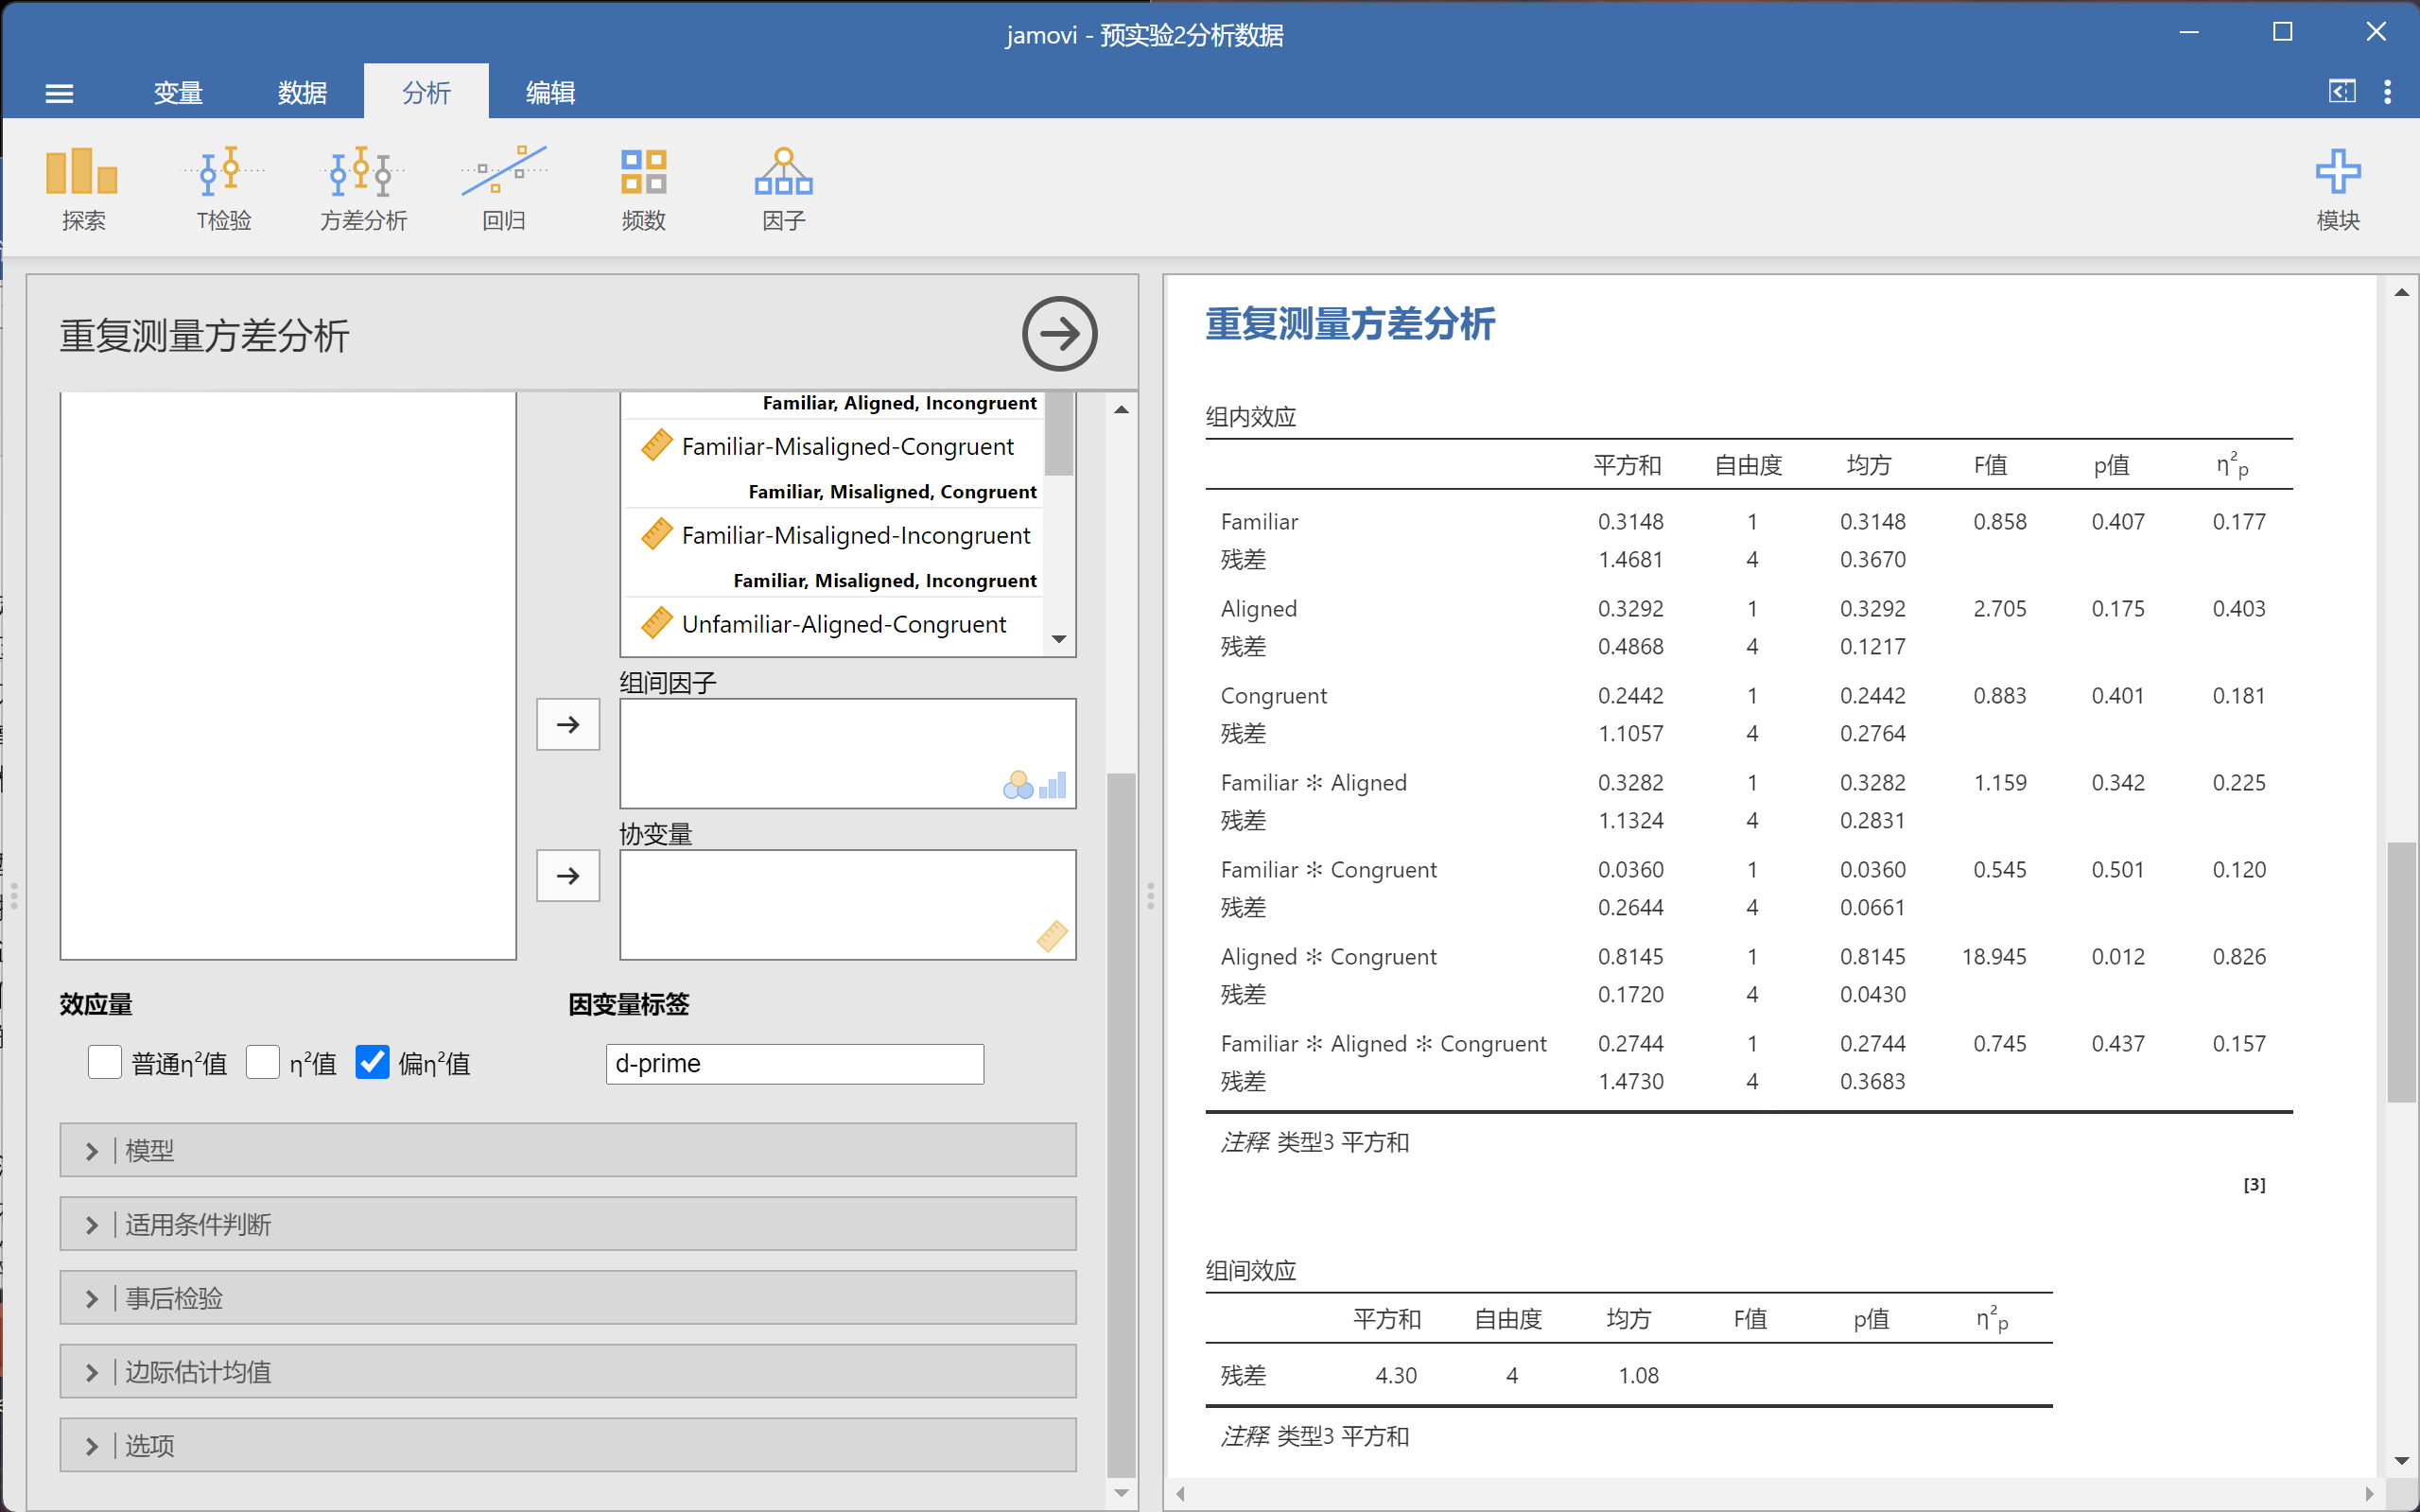
\includegraphics{img/jamovi/rmanova-result.png}

\section{简单效应分析}\label{ux7b80ux5355ux6548ux5e94ux5206ux6790}

这一部分承接上述重复测量方差分析。在本例中,当我们在jamovi中确定好了``重复测量因子''即``被试内变量''和``重复测量单元''即``实验条件''后,我们可以看到右侧的结果栏中就可以呈现统计结果,如果某两个或几个变量之间存在显著的交互作用,那么我们应当进行事后检验,以确定一个变量在与它有交互作用的另一个变量的哪些水平上显著,哪些水平上不显著。我们需要选择下列五个选项中的``事后检验''。

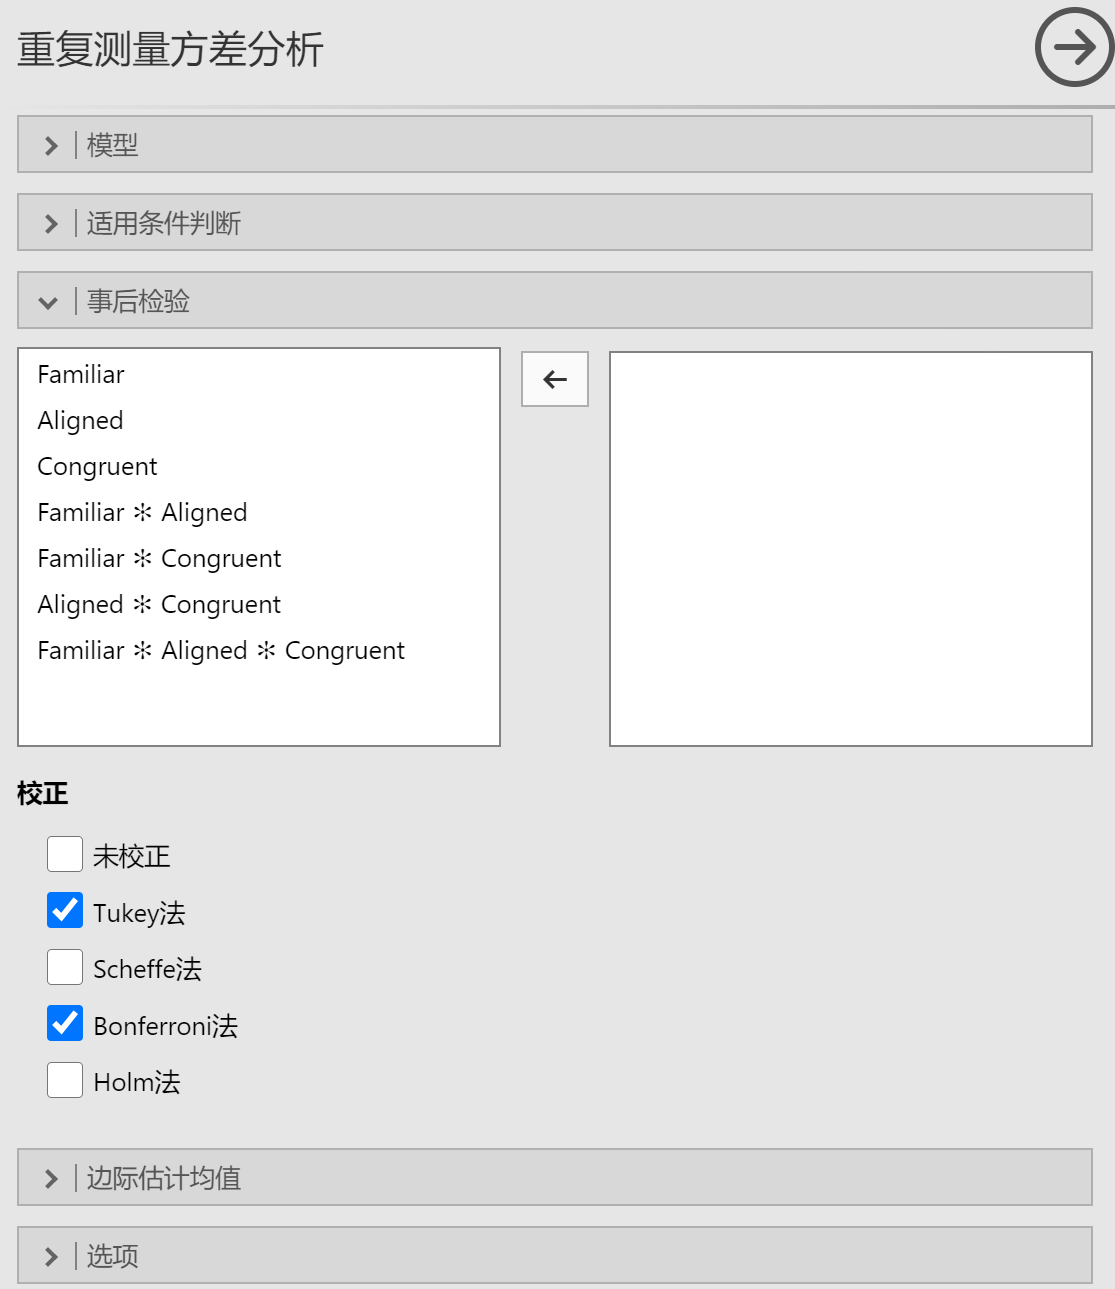
\includegraphics{img/jamovi/rmanova-posthoc.png}

选择需要进行事后检验的交互变量,并按照需要选择恰当的校正方法。

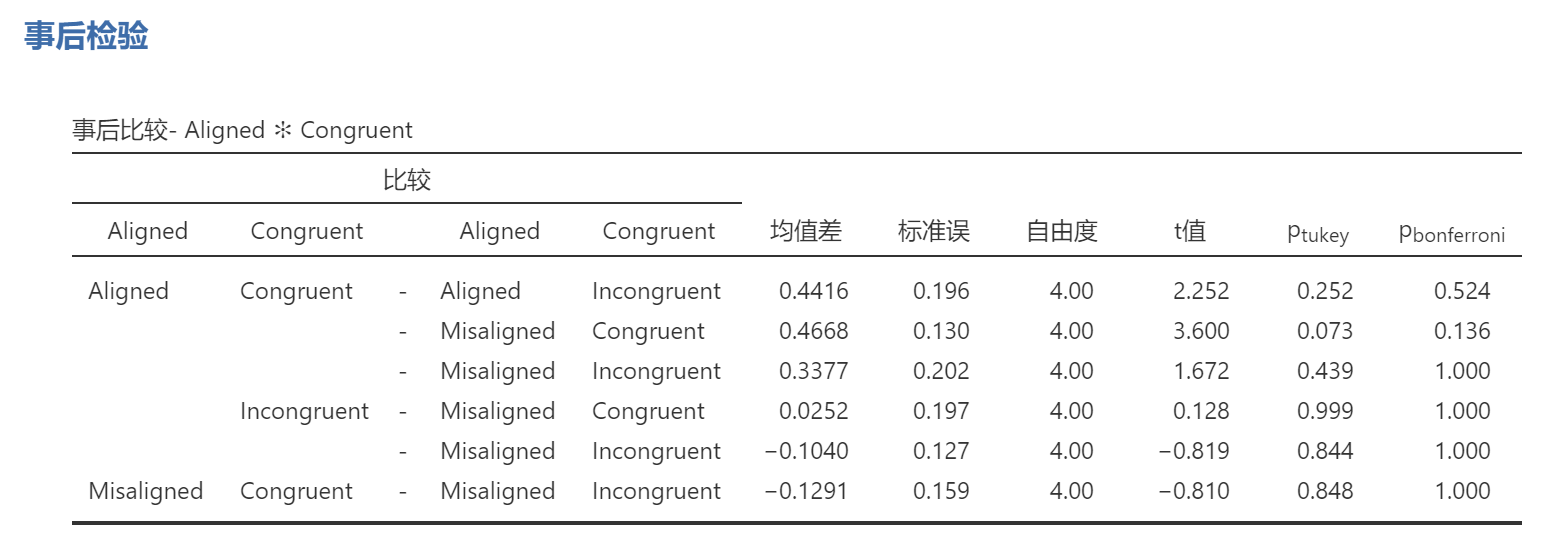
\includegraphics{img/jamovi/rmanova-posthoc-results.png}

右侧生成的结果的最右边两列就是jamovi按照我们选择的Tukey法和Bonferron法计算出的统计值。

\section{t检验}\label{tux68c0ux9a8c}

\begin{itemize}
\tightlist
\item
  首先,导入数据
\item
  其次,点击选项栏的分析,选择对应的t检验
\end{itemize}

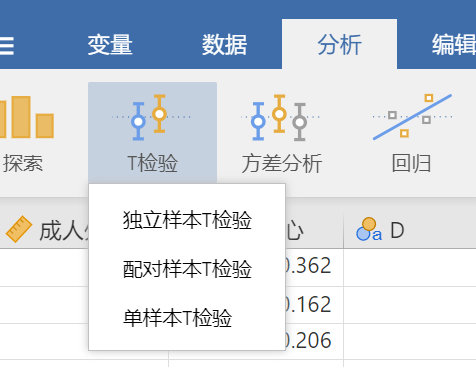
\includegraphics{img/jamovi/ttest.png}

\begin{itemize}
\tightlist
\item
  接着,选择要分析的变量
\end{itemize}

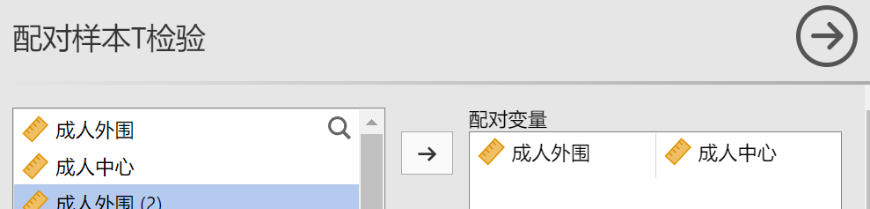
\includegraphics{img/jamovi/ttest-compare.png}

\begin{itemize}
\tightlist
\item
  然后,可以按需勾选,描述就是分析数据的均值、标准差、标准误等描述性数据;描述图就是生成图表
\end{itemize}

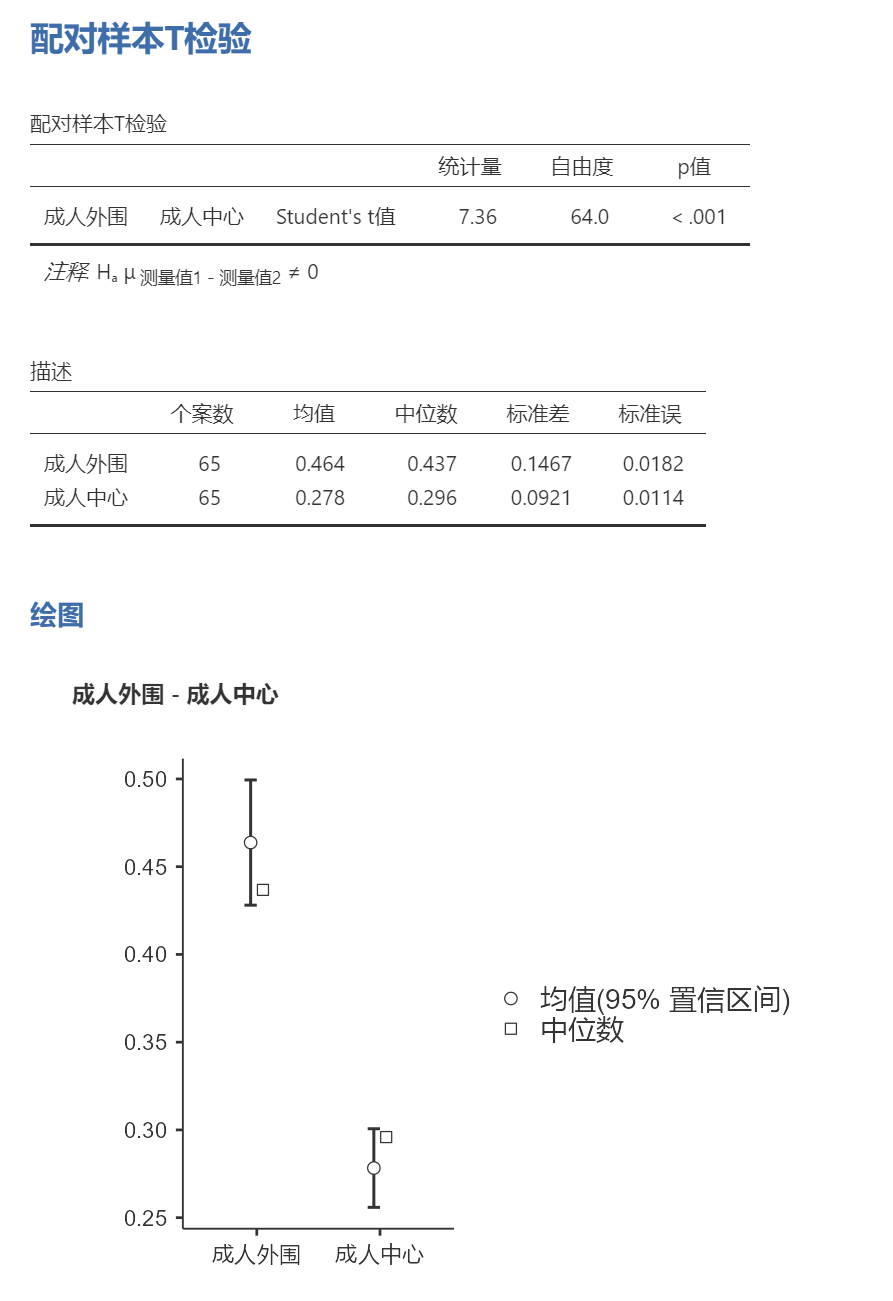
\includegraphics{img/jamovi/ttest-results.png}

\section{额外模块推荐}\label{ux989dux5916ux6a21ux5757ux63a8ux8350}

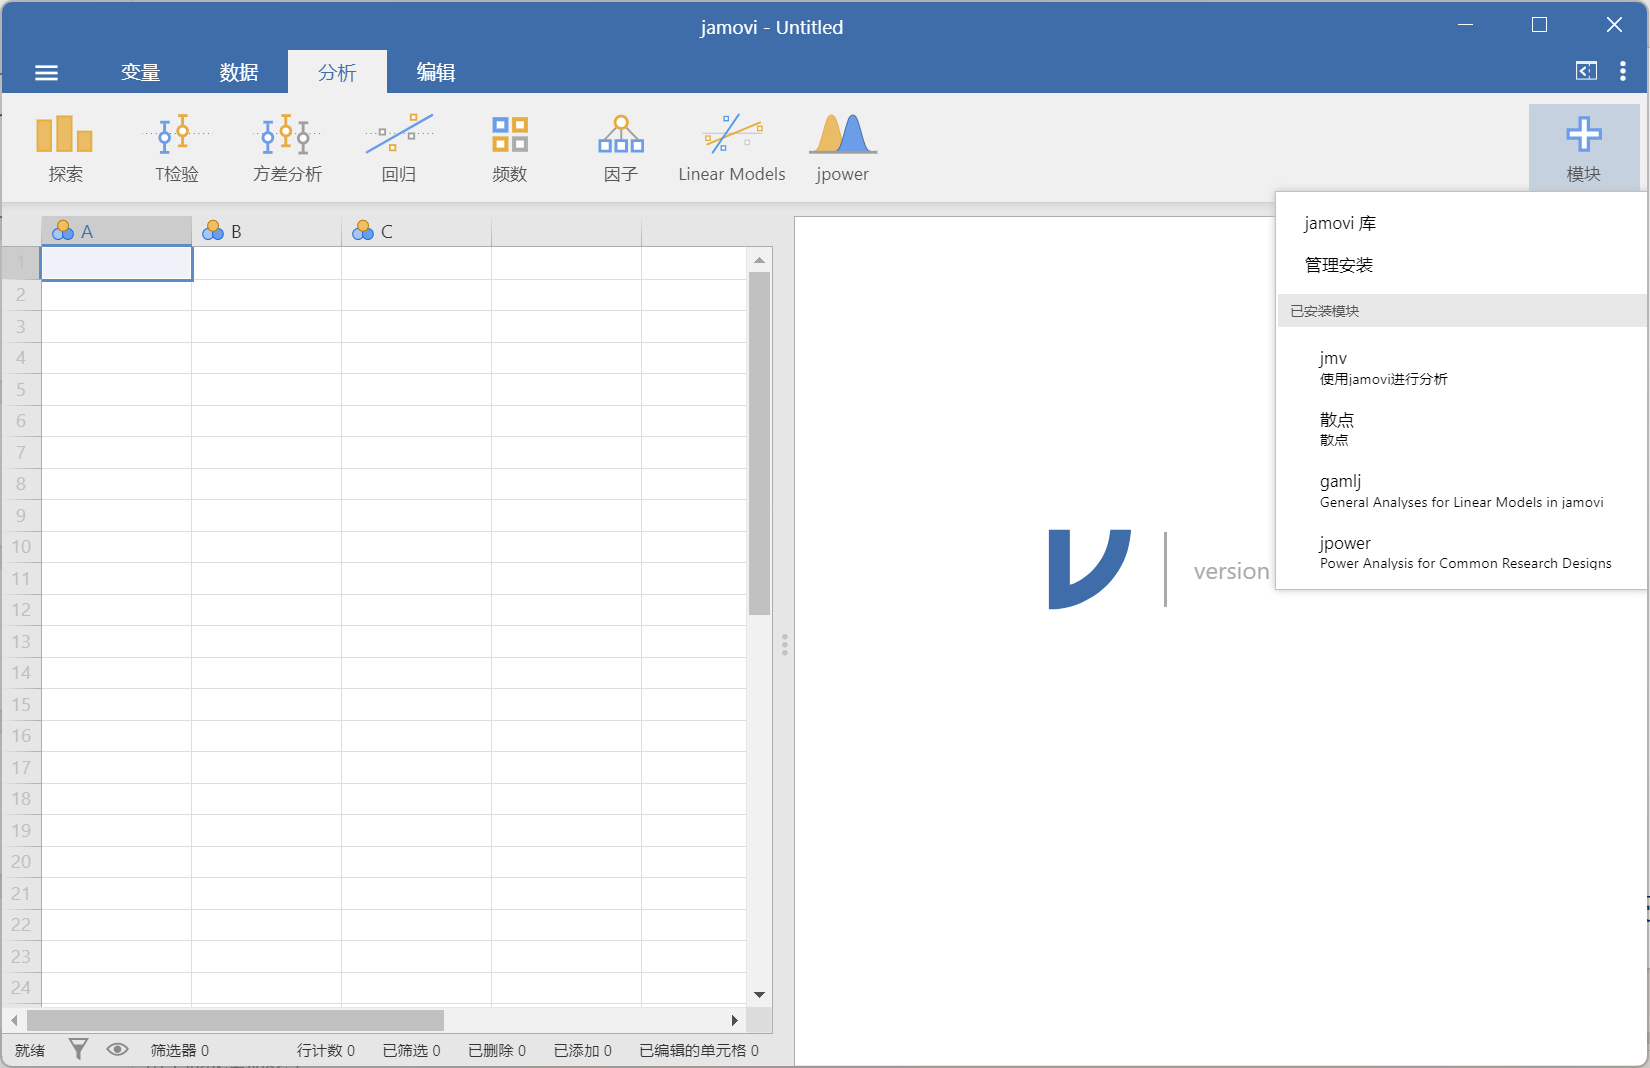
\includegraphics{img/jamovi/modules.png}\\
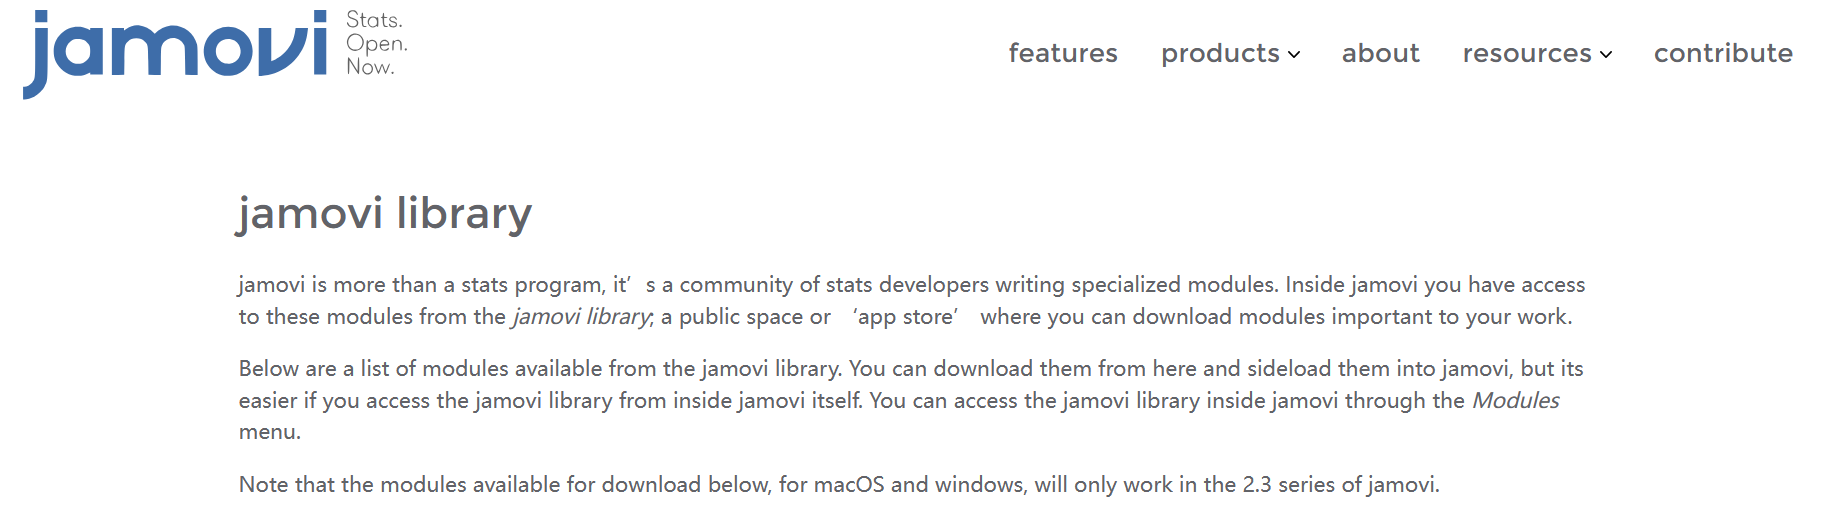
\includegraphics{img/jamovi/modules-library.png}

可以通过jamovi官网下载自己所需要的库。这是网址:\url{https://www.jamovi.org/library.html}

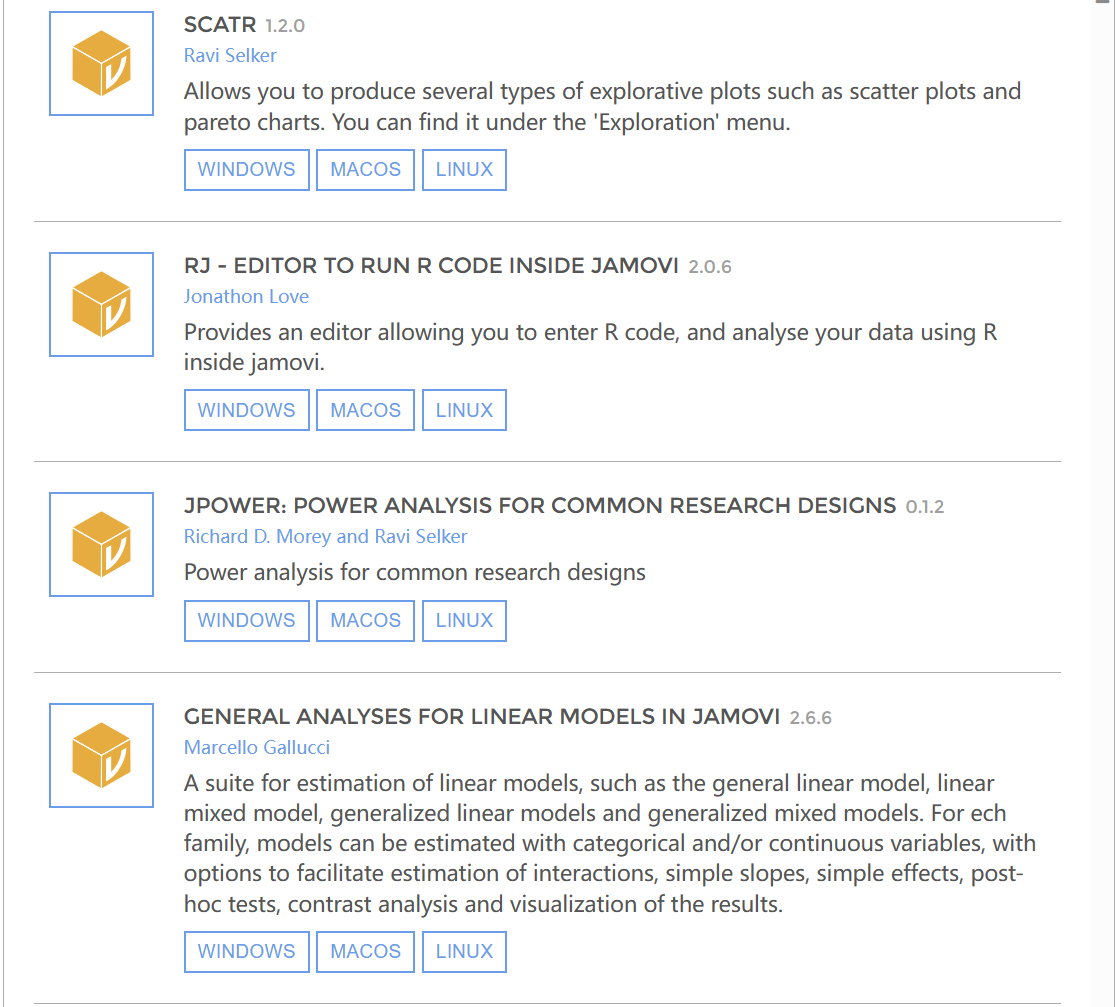
\includegraphics{img/jamovi/modules1.png}\\
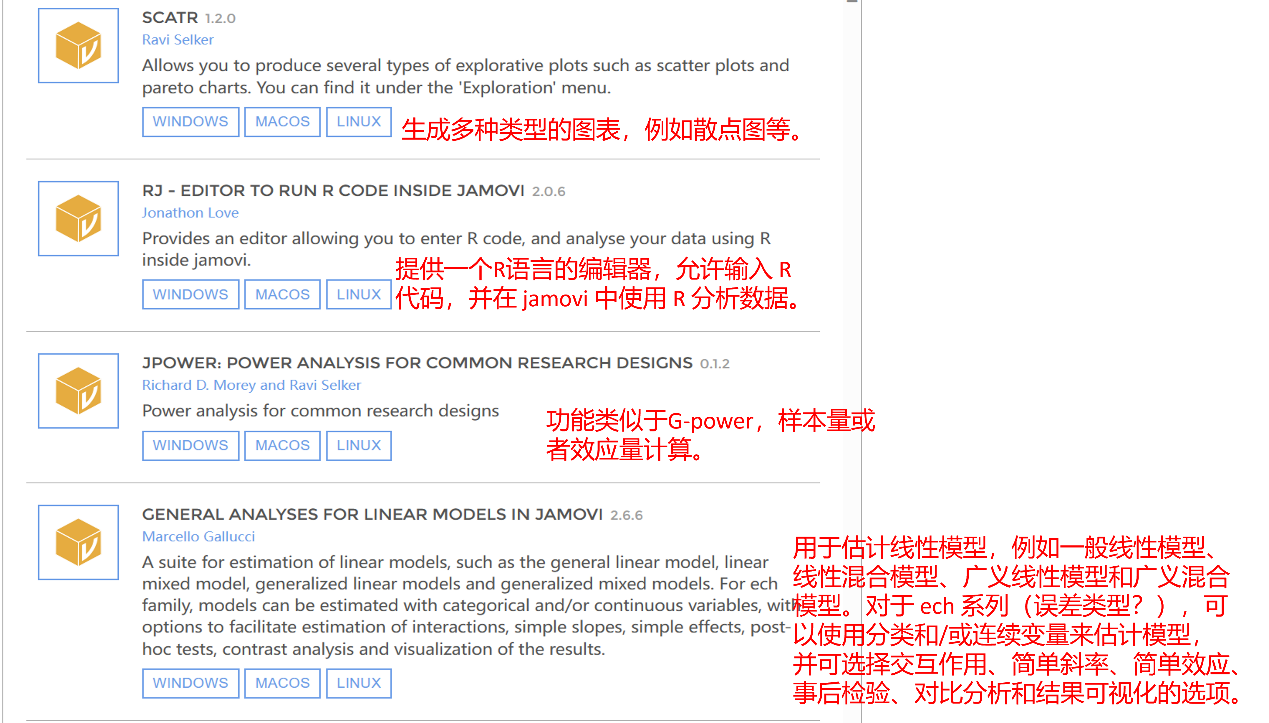
\includegraphics{img/jamovi/modules2.png}\\
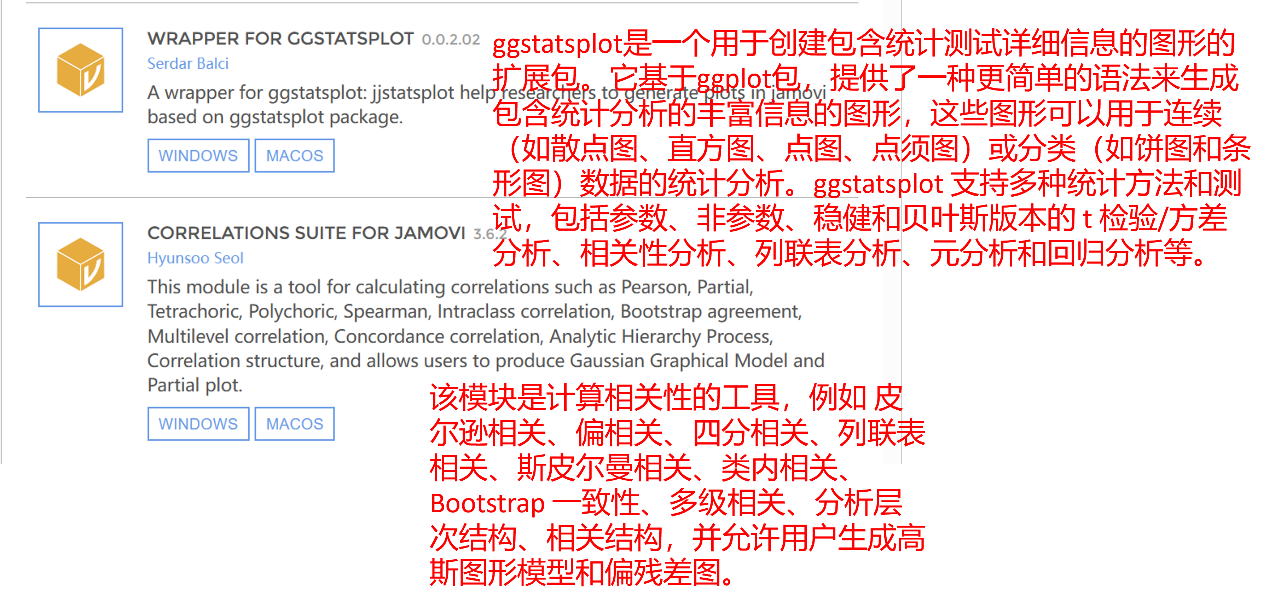
\includegraphics{img/jamovi/modules3.png}\\
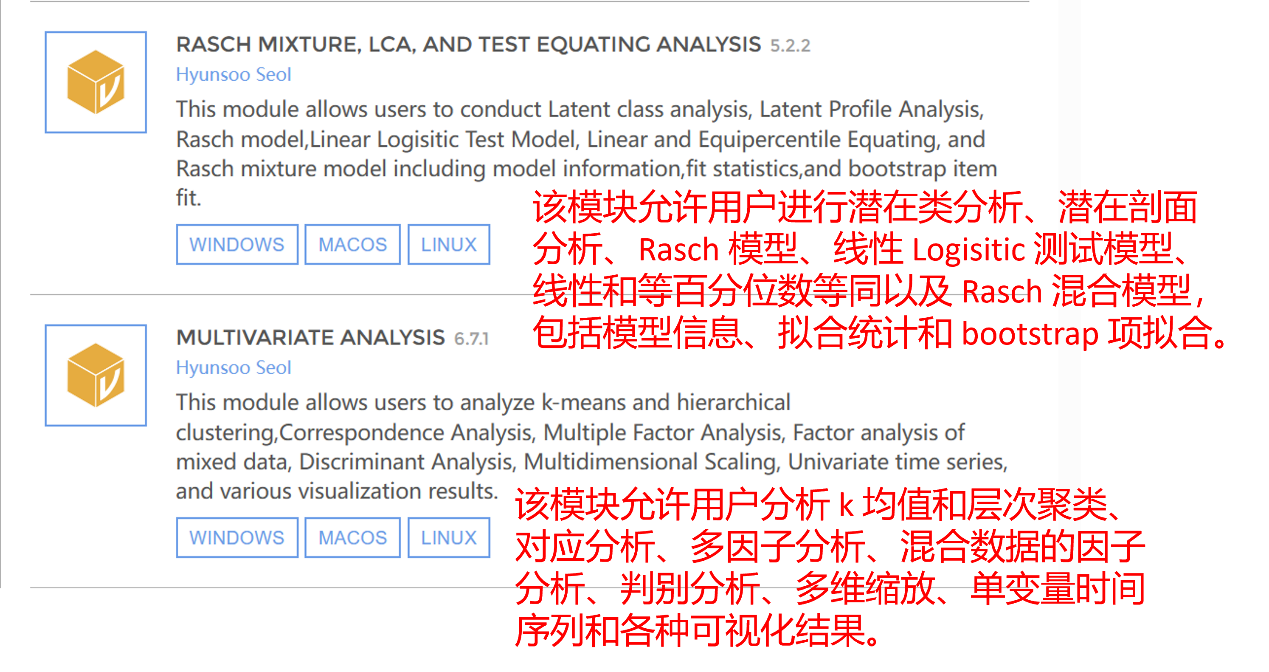
\includegraphics{img/jamovi/modules4.png}

\chapter{R语言}\label{r}

\section{预处理数据}\label{r-prepro}

汇总:
更新于:

\section{重复测量方差分析}\label{r-rm-anova}

汇总:
更新于:

\section{数据可视化}\label{r-plot}

汇总:
更新于:

\part{科研工具}\label{part-ux79d1ux7814ux5de5ux5177}

\chapter{Zotero}\label{zotero}

汇总:郭沫然\\
更新于:

\part{实验材料和公开数据}\label{part-ux5b9eux9a8cux6750ux6599ux548cux516cux5f00ux6570ux636e}

\chapter{实验材料}\label{materials}

汇总:\\
更新于:

\section{Chicago Face Database (芝加哥面孔数据库)}\label{chicago-face-database-ux829dux52a0ux54e5ux9762ux5b54ux6570ux636eux5e93}

\href{https://www.chicagofaces.org/}{Chicago Face Database}

Ma, D. S., Correll, J., \& Wittenbrink, B. (2015). The Chicago face database: A free stimulus set of faces and norming data. \emph{Behavior Research Methods}, 47(4), 1122--1135. \url{https://doi.org/10.3758/s13428-014-0532-5}

Ma, D. S., Kantner, J., \& Wittenbrink, B. (2021). Chicago Face Database: Multiracial expansion. \emph{Behavior Research Methods}, 53(3), 1289--1300. \url{https://doi.org/10.3758/s13428-020-01482-5}

\chapter{公开数据库}\label{opendata}

汇总:\\
更新于:

\section{磁共振(fMRI)}\label{ux78c1ux5171ux632ffmri}

\section{脑电(EEG)}\label{ux8111ux7535eeg}

\section{行为}\label{ux884cux4e3a}

\cleardoublepage

\appendix \addcontentsline{toc}{chapter}{\appendixname}


\chapter{如何为本手册作出贡献}\label{contribute}

如果你发现这个手册对你有帮助,欢迎你也贡献一份力量。如果你觉得这个手册没有什么用处,同样欢迎你提出建议,和我们一起来完善它。

\section{直接Pull Request}\label{ux76f4ux63a5pull-request}

如果你已经可以非常熟练地使用 Git 和 GitHub,那么你可以直接在 GitHub 上提交issues或Pull Request。

\section{简易教程}\label{ux7b80ux6613ux6559ux7a0b}

如果你对 Git 和 GitHub 不太熟悉,也请不到担心,你仍然可以通过本教程,学习如何完成一个可以成为本手册一部分的Rmd文件。完成后你只需将新创建的Rmd文档发送给我们,审核通过后该文档内容就会出现在\href{https://haiyangjin.github.io/labbook/}{本实验室手册}。

\subsection{下载示例}\label{ux4e0bux8f7dux793aux4f8b}

首先请下载\href{https://github.com/HaiyangJin/labbook/archive/refs/heads/mini.zip}{示例}。解压后你会看到一个名为\texttt{labbook-mini}的文件夹。

\begin{figure}

{\centering 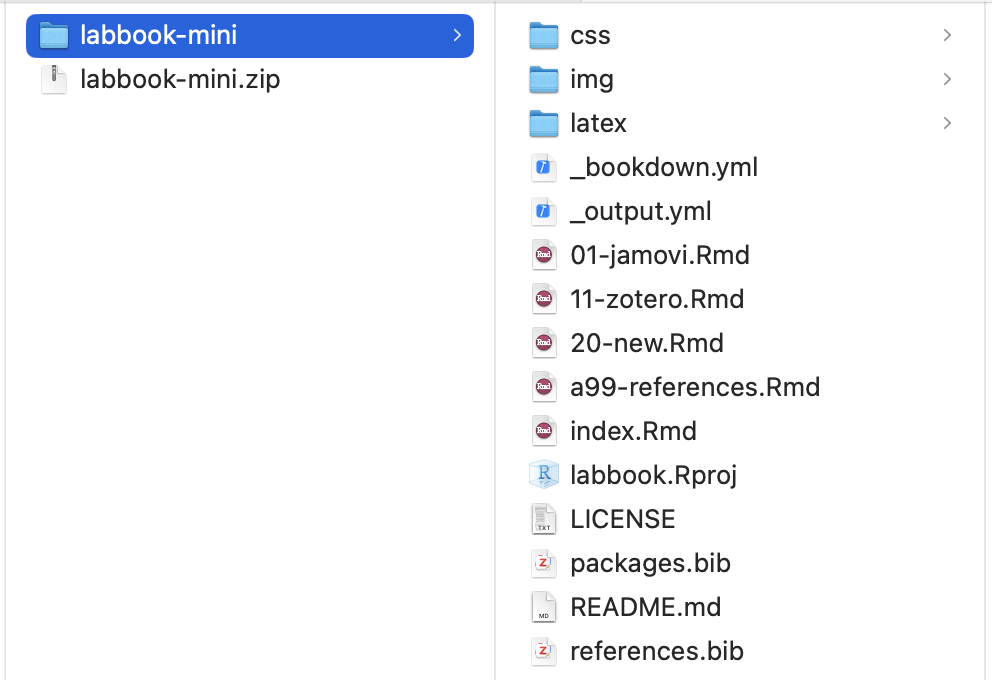
\includegraphics[width=0.7\linewidth]{img/contribute/mini_dir} 

}

\caption{The minimal example directory}\label{fig:contri-mini-dir}
\end{figure}

\subsection{安装R和RStudio}\label{ux5b89ux88c5rux548crstudio}

如果你还没有安装R和RStudio,请先根据\href{https://haiyangjin.github.io/rpsych-cn/intro.html\#prepare}{这里的信息}安装相关软件以及进行相应的设置。

安装完成后,请不要忘了\href{https://haiyangjin.github.io/rpsych-cn/intro.html\#mirror}{设置R包的镜像源}。

完成后请安装bookdown包,可以在RStudio中运行以下代码来实现:

\begin{Shaded}
\begin{Highlighting}[]
\FunctionTok{install.packages}\NormalTok{(}\StringTok{"bookdown"}\NormalTok{)}
\end{Highlighting}
\end{Shaded}

如果遇到问题,可以尝试查看这里的\href{https://haiyangjin.github.io/rpsych-cn/qacn.html\#qacn}{帮助信息}。

\subsection{打开labbook.Rproj}\label{ux6253ux5f00labbook.rproj}

请\textbf{直接}双击\texttt{labbook-mini}文件夹中的\texttt{labbook.Rproj}文件,这样你就可以在RStudio中打开这个项目。

\begin{quote}
请\textbf{直接}双击\texttt{labbook-mini}文件夹中的\texttt{labbook.Rproj}文件,这样你就可以在RStudio中打开这个项目。
\end{quote}

\begin{theorem}
请\textbf{直接}双击\texttt{labbook-mini}文件夹中的\texttt{labbook.Rproj}文件,这样你就可以在RStudio中打开这个项目。
\end{theorem}

打开后你会看到如下的界面:

\begin{figure}

{\centering 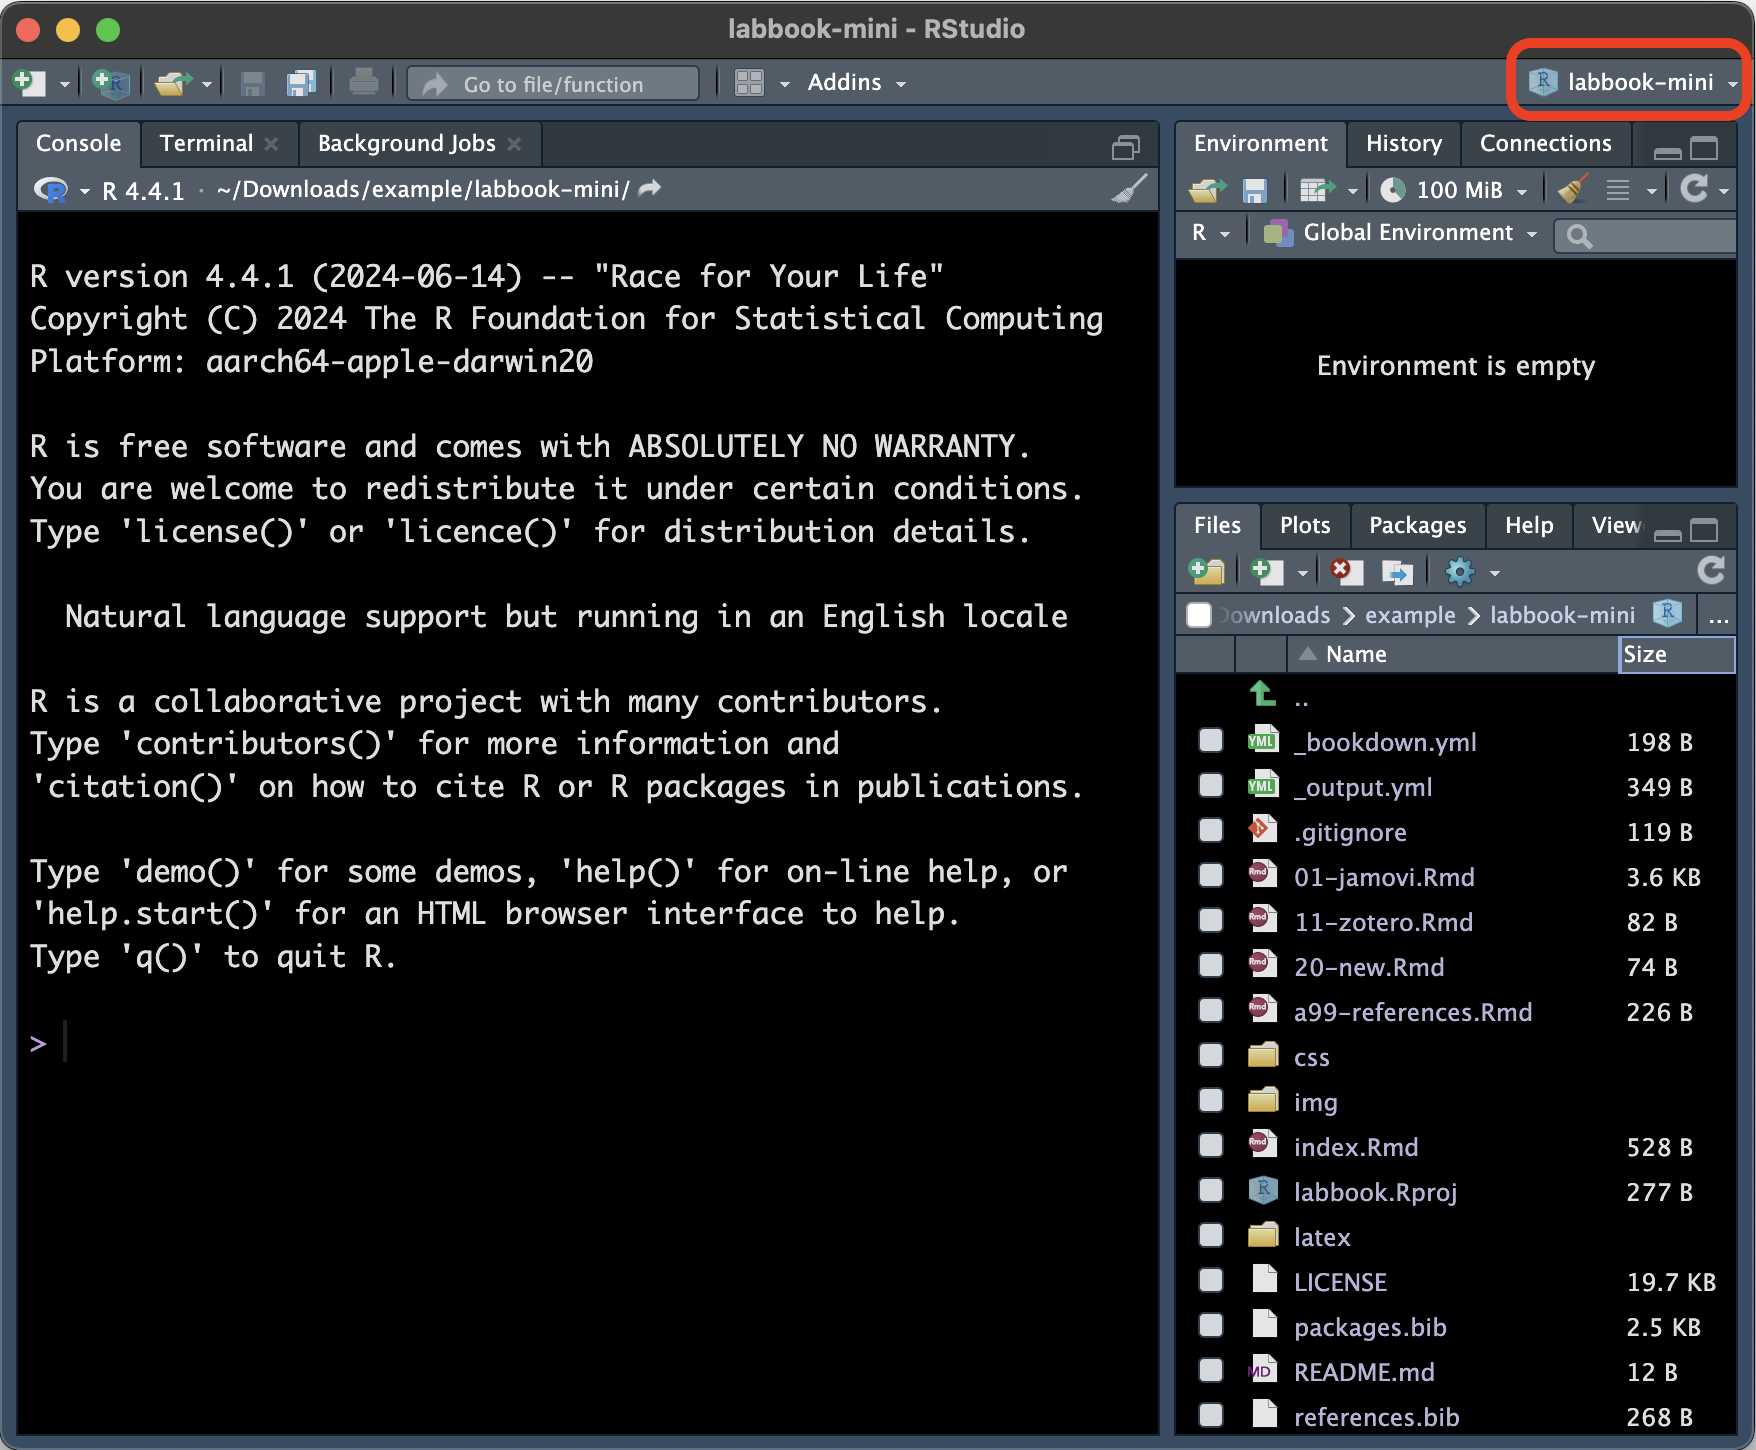
\includegraphics[width=0.9\linewidth]{img/contribute/mini_rproj} 

}

\caption{The minimal example R project}\label{fig:contri-mini-rproj}
\end{figure}

\textcolor{red}{\textbf{特别注意}}:请确保如上图 \ref{fig:contri-mini-rproj}右上角所示,当前的项目名称是\texttt{labbook-mini}。如果不是,请点击\texttt{File} -\textgreater{} \texttt{Open\ project...},然后选择\texttt{labbook-mini}文件夹中的\texttt{labbook.Rproj}文件,重新打开该项目。

\subsection{确认示例可以运行}\label{ux786eux8ba4ux793aux4f8bux53efux4ee5ux8fd0ux884c}

现在我们可以尝试运行这个示例了。请在RStudio右上角找到\texttt{Build},然后点击\texttt{Build\ Book}。如果一切顺利,会跳出一个窗口,同时你应该会在RStudio的右上角看到:

\begin{figure}

{\centering 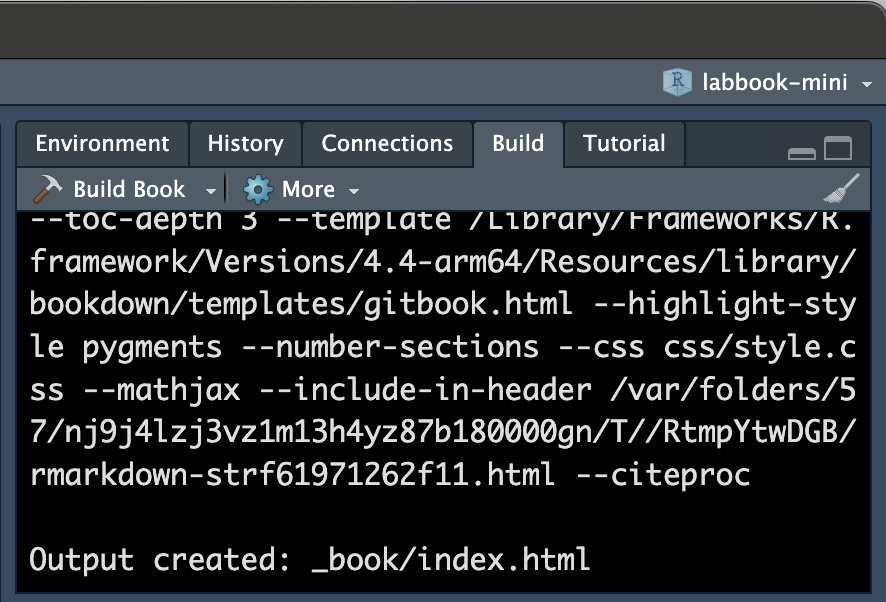
\includegraphics[width=0.7\linewidth]{img/contribute/mini_build} 

}

\caption{Build book for the minimal example}\label{fig:contri-mini-build}
\end{figure}

如果你不小心关掉了跳出的窗口,你应该会看到在\texttt{labbook-mini}文件夹中生成了一个\texttt{\_book}子文件夹,里面包含了一个\texttt{index.html}文件。请双击这个文件通过浏览器打开,你会看到一个网页版的示例。

\subsection{创建一个新的Rmd文件}\label{ux521bux5efaux4e00ux4e2aux65b0ux7684rmdux6587ux4ef6}

现在我们可以开始创建一个新的Rmd文件来介绍你想贡献的内容了。比如你可以打开\texttt{20-new.Rmd}文件,然后将其另存为\texttt{66-your\_topic.Rmd}。请确保你的文件名中包含了你的主题,这样我们可以更容易地了解不同\texttt{Rmd}文件的内容。

例如,你可以输入这些内容:

\begin{Shaded}
\begin{Highlighting}[]
\FunctionTok{\# 我的主题}

\InformationTok{    汇总:最棒的我     }
\InformationTok{    更新于:很开心的今天(或者2024年11月11日)}

\InformationTok{    就是想分享一下今天的快乐。。。}

\FunctionTok{\#\# 加一个二级标题}


\FunctionTok{\#\#\# 需要放一张照片}

\SpecialStringTok{{-} }\NormalTok{添加图片方式一:}
\InformationTok{\textasciigrave{}\textasciigrave{}\textasciigrave{}\{r test{-}my{-}topic, echo=FALSE, fig.cap=\textquotesingle{}我的图片\textquotesingle{}, out.width=\textquotesingle{}60\%\textquotesingle{}, fig.align=\textquotesingle{}center\textquotesingle{}\}}
\InformationTok{knitr::include\_graphics(file.path("img", "jamovi", "anova.png"))}
\InformationTok{\textasciigrave{}\textasciigrave{}\textasciigrave{}}

\SpecialStringTok{{-} }\NormalTok{添加图片方式二:}
\AlertTok{![](img/jamovi/modules{-}library.png)}

\FunctionTok{\#\# 再给文字加一些颜料}

\NormalTok{随随便便放一些文字,看看效果如何。}

\NormalTok{我还想再给某一些文字加个链接,比如}\CommentTok{[}\OtherTok{这里}\CommentTok{](https://www.jamovi.org/)}\NormalTok{。}
\NormalTok{或者再加一些特定的颜色,比如}\CommentTok{[}\OtherTok{红色}\CommentTok{]}\NormalTok{\{color="red"\}和}\CommentTok{[}\OtherTok{蓝色}\CommentTok{]}\NormalTok{\{color="green"\},}
\CommentTok{[}\OtherTok{对的,}\CommentTok{]}\NormalTok{\{color="\#5bc0eb"\}}\CommentTok{[}\OtherTok{我就是}\CommentTok{]}\NormalTok{\{color="\#fa7921"\}}\CommentTok{[}\OtherTok{想弄个}\CommentTok{]}\NormalTok{\{color="\#9bc53d"\}}
\CommentTok{[}\OtherTok{Stroop效应}\CommentTok{]}\NormalTok{\{color="\#e55934"\}(抱歉,颜色有点丑)。}

\FunctionTok{\#\#\# 再来一个列表}

\SpecialStringTok{{-} }\NormalTok{一个}
\SpecialStringTok{{-} }\NormalTok{两个}
\SpecialStringTok{{-} }\NormalTok{三个}

\SpecialStringTok{1. }\NormalTok{第一个}
\SpecialStringTok{2. }\NormalTok{第二个}
\SpecialStringTok{3. }\NormalTok{第三个}
\end{Highlighting}
\end{Shaded}

\subsection{重新Build book}\label{ux91cdux65b0build-book}

输入一些Rmarkdown内容后,请通过RStudio右上角的\texttt{Build},再一次\texttt{Build\ Book}及时检查是否可以成功生成网页文件。\textcolor{red}{如果你已经输入了上述所有代码,那你应该会看到}:

\begin{figure}

{\centering 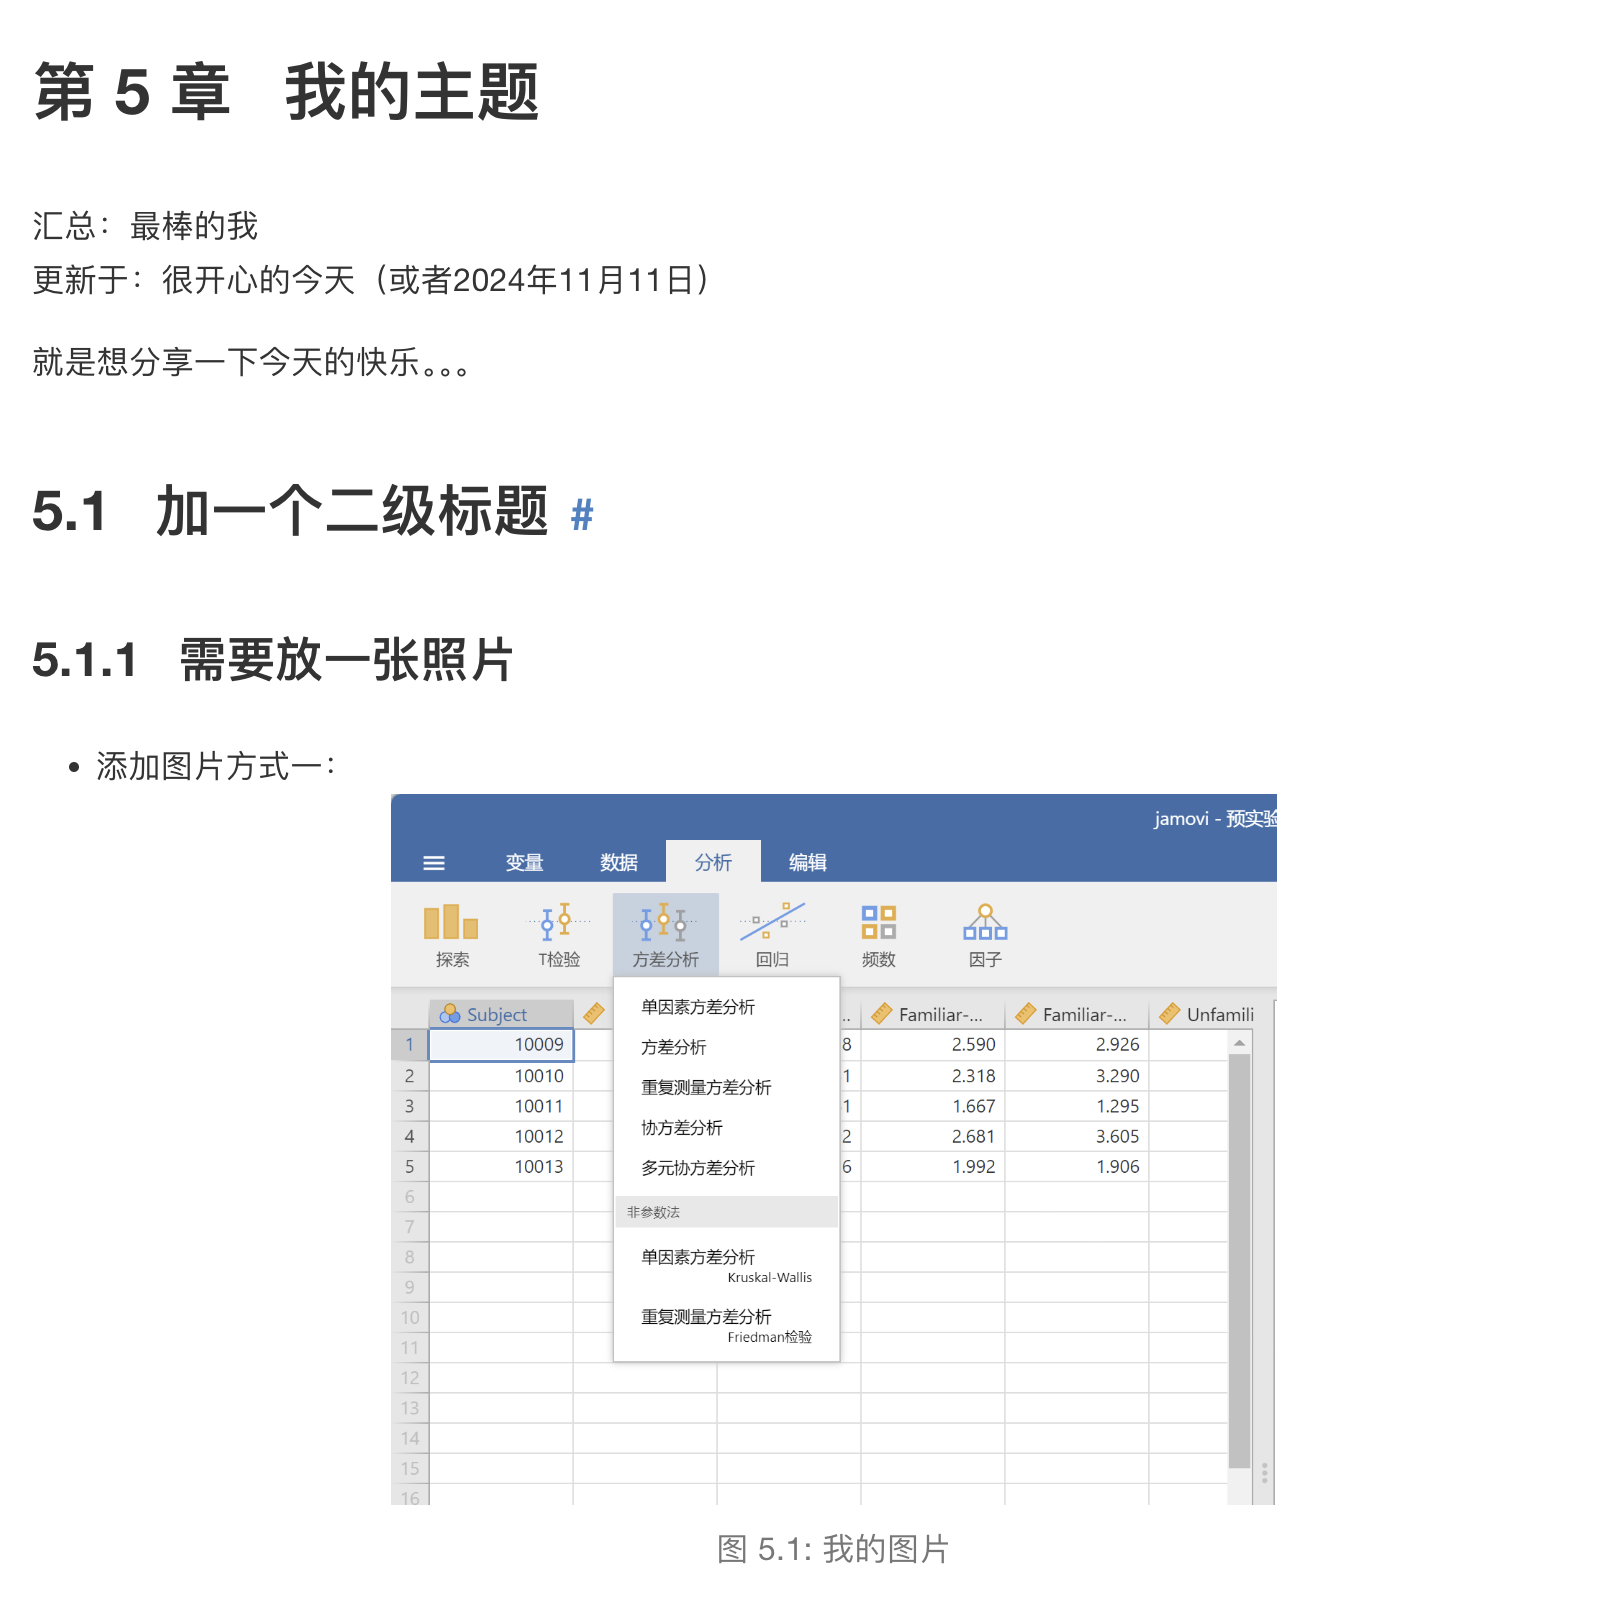
\includegraphics[width=0.8\linewidth]{img/contribute/new_rmd_output1} 

}

\caption{The new Rmd file output}\label{fig:contri-new-rmd-1}
\end{figure}
\begin{figure}

{\centering 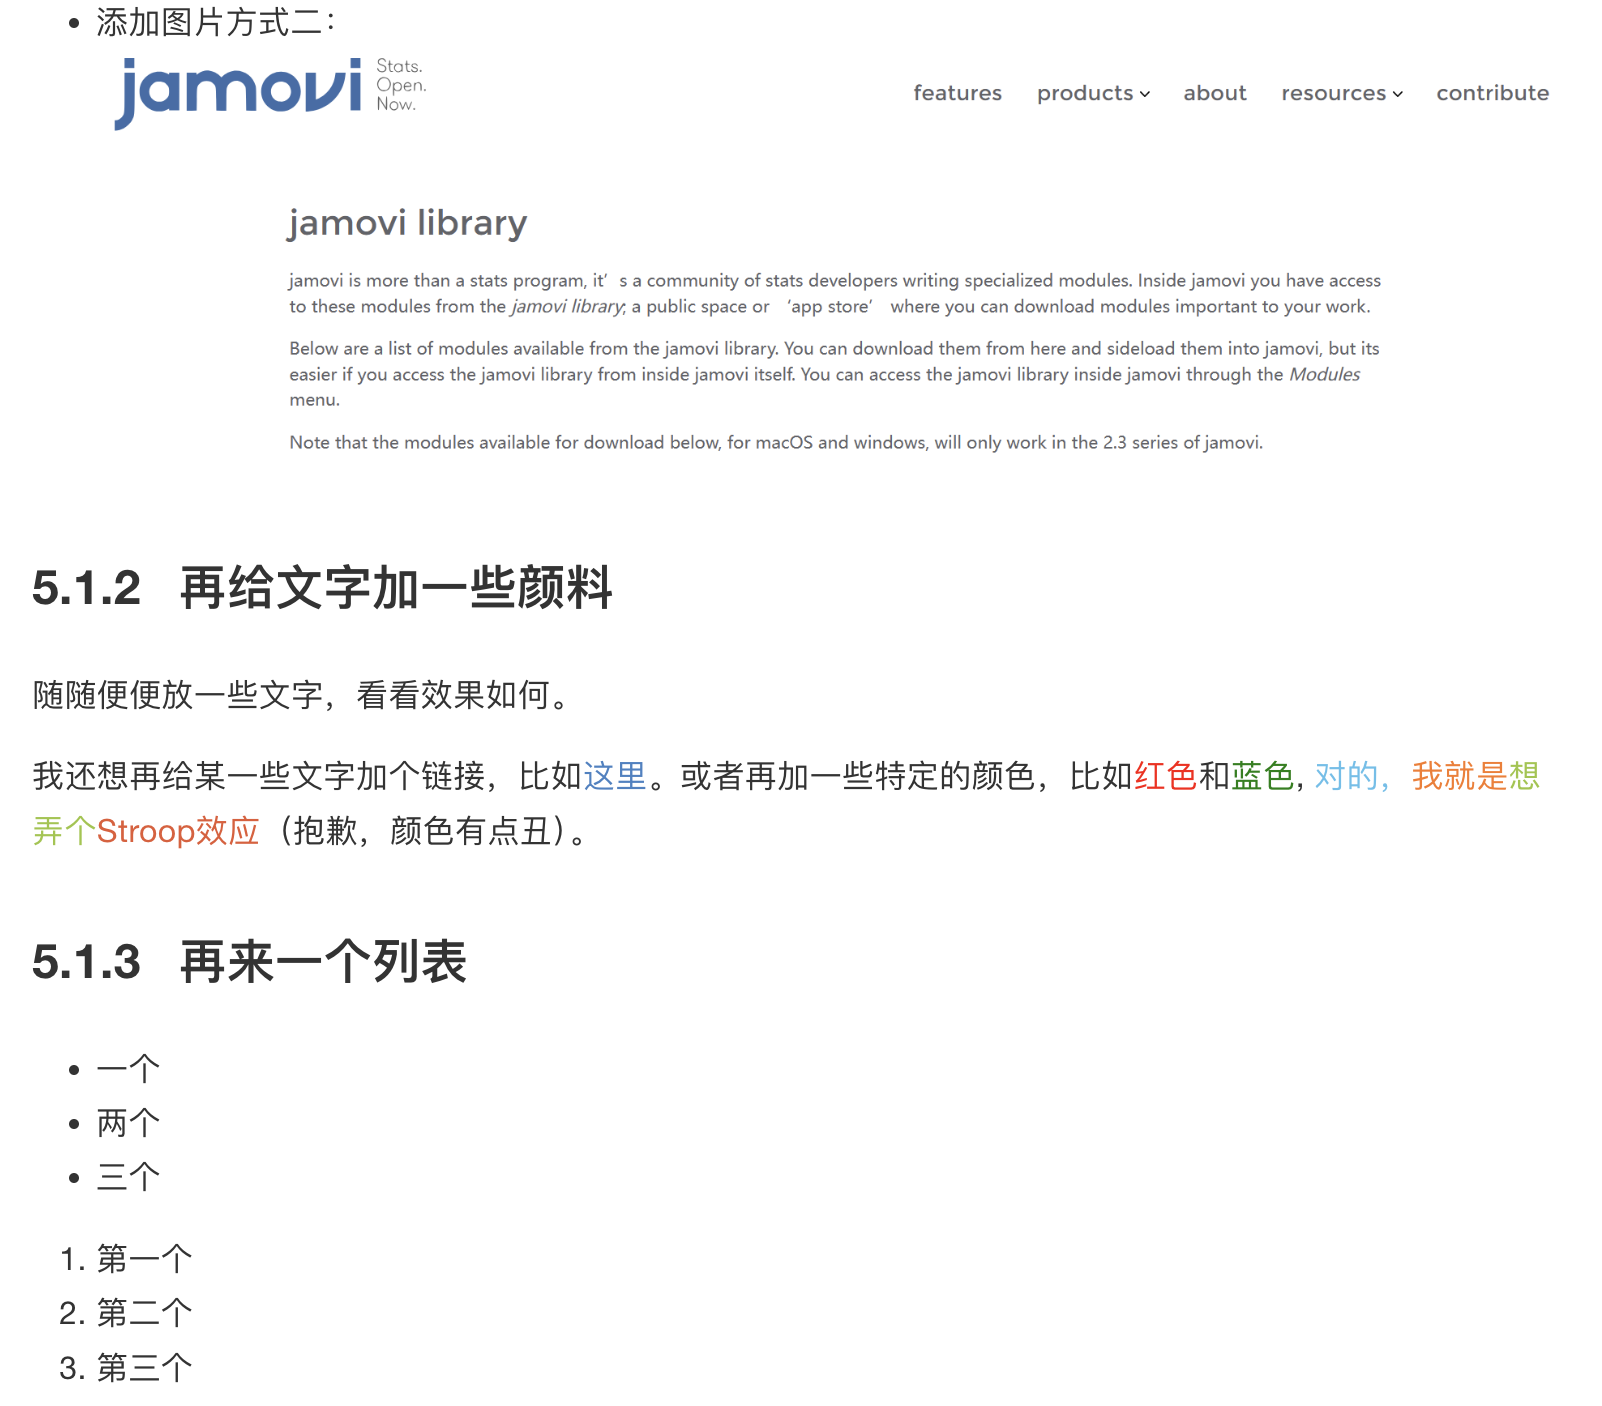
\includegraphics[width=0.8\linewidth]{img/contribute/new_rmd_output2} 

}

\caption{The new Rmd file output}\label{fig:contri-new-rmd-2}
\end{figure}

\subsection{其他}\label{ux5176ux4ed6}

如果你想再了解其他关于Rmarkdown/markdown的一些``特殊''用法,可以看看\href{https://bookdown.org/yihui/bookdown/markdown-syntax.html\#block-level-elements}{这里}。

就先这样吧。如果你有任何问题,欢迎随时联系\href{https://haiyangjin.github.io/en/contact/}{我们}。

期待着你的Rmd会出现在手册里!

\chapter{常见问题}\label{qa}

\section{R和RStudio相关问题}\label{rux548crstudioux76f8ux5173ux95eeux9898}

有关R和RStudio的相关问题请查看\href{https://haiyangjin.github.io/rpsych-cn/qacn.html\#qacn}{这里}。

\section{格式调整}\label{ux683cux5f0fux8c03ux6574}

\subsection{文字}\label{ux6587ux5b57}

\subsubsection{文字颜色}\label{ux6587ux5b57ux989cux8272}

你可以通过以下代码设置文字的颜色:

\begin{Shaded}
\begin{Highlighting}[]
\CommentTok{[}\OtherTok{红色}\CommentTok{]}\NormalTok{\{color="red"\}   }
\CommentTok{[}\OtherTok{蓝色}\CommentTok{]}\NormalTok{\{color="green"\}  }
\CommentTok{[}\OtherTok{绿色}\CommentTok{]}\NormalTok{\{color="blue"\}  }
\CommentTok{[}\OtherTok{黄色}\CommentTok{]}\NormalTok{\{color="yellow"\}}
\end{Highlighting}
\end{Shaded}

相应的显示为:\\
\textcolor{red}{红色}\\
\textcolor{green}{蓝色}\\
\textcolor{blue}{绿色}\\
\textcolor{yellow}{黄色}

\subsection{图片}\label{ux56feux7247}

强烈建议使用以下格式显示图片,这样可以灵活的设置图片的大小和位置等。

\begin{Shaded}
\begin{Highlighting}[]
\InformationTok{\textasciigrave{}\textasciigrave{}\textasciigrave{}\{r test{-}my{-}topic, echo=FALSE, fig.cap=\textquotesingle{}我的图片\textquotesingle{}, out.width=\textquotesingle{}60\%\textquotesingle{}, fig.align=\textquotesingle{}center\textquotesingle{}\}}
\InformationTok{knitr::include\_graphics(file.path("img", "jamovi", "anova.png"))}
\InformationTok{\textasciigrave{}\textasciigrave{}\textasciigrave{}}
\end{Highlighting}
\end{Shaded}

\begin{figure}

{\centering 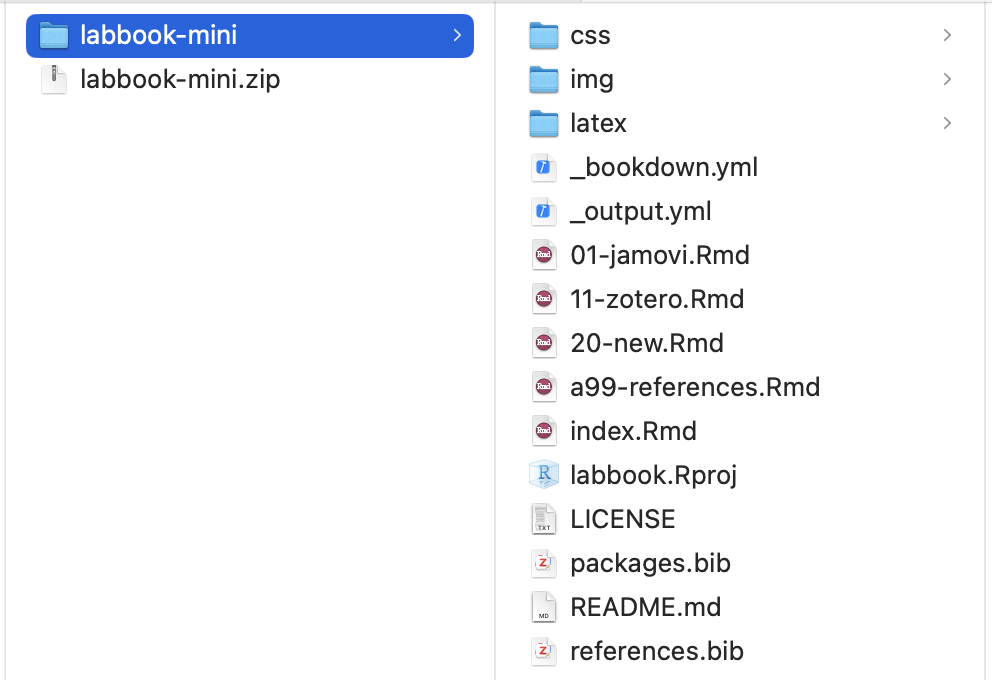
\includegraphics[width=0.7\linewidth]{img/contribute/mini_dir} 

}

\caption{这是描述图片的题目}\label{fig:qa-img-run}
\end{figure}

\begin{itemize}
\tightlist
\item
  \texttt{qa-img}:图片的名称,可以自定义(但请不能在同一个文档中重复)。该名称也可以通过 \texttt{\textbackslash{}@ref(fig:qa-img)} 引用该图片,如\texttt{\textbackslash{}@ref(fig:qa-img)}。
\item
  \texttt{echo=TRUE}:是否显示该 R chunk 代码。一般情况下应设为 \texttt{FALSE}。这里为了展示代码,所以设为 \texttt{TRUE}。
\item
  \texttt{fig.cap=\textquotesingle{}这是描述图片的题目\textquotesingle{}}:图片的题目。
\item
  \texttt{out.width=\textquotesingle{}70\%\textquotesingle{}}:图片的宽度,可以设置为百分比或者像素。
\item
  \texttt{fig.align=\textquotesingle{}center\textquotesingle{}}:图片的位置,可以设置为 \texttt{center}、\texttt{left} 或者 \texttt{right}。
\end{itemize}

\bibliography{references.bib,packages.bib}

\backmatter
\printindex

\end{document}
